\documentclass[10pt]{article}

\usepackage[margin=0.82in,top=0.85in,bottom=0.85in]{geometry}
\usepackage[T1]{fontenc}
\usepackage{lmodern}
\usepackage[scaled=0.84]{beramono}
\usepackage{microtype}
\usepackage{amsmath,amssymb}
\usepackage{booktabs}
\usepackage{tabularx}
\usepackage{array}
\usepackage{multirow}
\usepackage{enumitem}
\usepackage{xcolor}
\usepackage{natbib}
\setcitestyle{authoryear,round,citesep={;},aysep={,},yysep={;}}
\usepackage{tikz}
\usetikzlibrary{arrows.meta,positioning,fit,shapes.geometric,calc}
\usepackage[colorlinks=true,linkcolor=navy,citecolor=tealdark,urlcolor=navy]{hyperref}

\emergencystretch=2.5em
\setlength{\parskip}{0.42em}
\setlength{\parindent}{0pt}

\definecolor{navy}{HTML}{1B365D}
\definecolor{tealdark}{HTML}{0E6B6B}
\definecolor{slate}{HTML}{475569}
\definecolor{bgsoft}{HTML}{F8FAFC}
\definecolor{warnamber}{HTML}{B45309}
\definecolor{alertred}{HTML}{991B1B}
\definecolor{okgreen}{HTML}{166534}
\definecolor{accentblue}{HTML}{2563EB}
\definecolor{accentorange}{HTML}{D97706}
\definecolor{accentpurple}{HTML}{6D28D9}

\newcolumntype{Y}{>{\raggedright\arraybackslash}X}
\newcommand{\code}[1]{\texttt{#1}}
\newcommand{\holdbadge}{\textbf{\textcolor{alertred}{[HOLD]}}}
\newcommand{\na}{\textit{N/A}}

\newenvironment{conceptbox}[1]{%
  \par\vspace{4pt}\noindent\begin{tikzpicture}%
  \node[draw=navy!45, fill=bgsoft, rounded corners=3pt, inner sep=7pt, text width=\dimexpr\linewidth-16pt\relax, align=left] (box) \bgroup%
  {\small\textbf{\textcolor{navy}{#1}}\par\vspace{2pt}\footnotesize}%
}{%
  \egroup;\end{tikzpicture}\par\vspace{4pt}%
}

\begin{document}

\title{\vspace{-1.0em}\textbf{\Large Evidence-Gated Telemetry Auditing and Context-Boundary Reconstruction\\for Long-Horizon Tool-Using LLM Agents: A Case Study on Project HINAGI}}

\author{Seungwon Lee \\
\small Independent Researcher \\
\small \texttt{redcar1024@gmail.com}}

\date{November 2026}
\sloppy
\maketitle

\begin{abstract}
Scalar leaderboard scores in long-horizon interactive agent benchmarks routinely conceal heterogeneous runtime pathologies---right-censored network timeouts, silent prompt mutations that invalidate prefix caches, concurrent configuration drift, and unrecorded serving eviction events. Building on reproducibility and agent-context evaluation scholarship \citep{kapoor2025ai,siegel2025corebench,lindenbauer2025complexity}, we develop and apply an \textbf{Evidence-Gated Telemetry Auditing Protocol} that binds every empirical claim to four hash-verified local evidence tiers (\code{E1-SOURCE}, \code{E2-CONFIG}, \code{E3-LOCAL-LOG}, \code{E4-OFFLINE}) while quarantining unarchived external submissions in a strict zero-citation \code{HOLD} state. Exercising this six-stage protocol on Project HINAGI's 25-game public-split ARC-AGI-3 evaluation (\code{V10}) and an earlier configuration smoke run (\code{V6}) yields four bounded methodological and empirical findings. First, \textbf{three-scope client token reconciliation without cross-plane imputation} closes to exact zero discrepancy across all 25 games: action-attributed history tokens (\code{378,304}) omit trailing non-action outputs captured in per-game logs (\code{468,510}, \code{86.23\%} reasoning tokens) and one detached root fallback record (\code{471,288} full client completions), while \code{4} HTTP read timeouts are isolated as right-censored \na{} rather than conflated with server-side completions (\code{7,610} output tokens) or stop-token offsets. Second, \textbf{deterministic execution-order boundary replay} reproduces all \code{177/177} post-initial prompt boundaries under a \code{44,544}-token budget, showing how character-to-token estimator clamping and two-phase prompt mutation split \code{9} evicted runs into \code{4} turn-end trims and \code{5} next-turn opener trims. Third, \textbf{clustered prefix-cache stratification} across \code{N=24/25} games documents sharp contrasts between pure-append reuse (\code{88.52\%} pooled) and host-mutated transitions (\code{15.53\%} pooled / \code{17.18\%} game-pooled on image scrubbing; \code{18.12\%} on FIFO deletion, totaling \code{75.37\%} of uncached prefill), while explicitly withholding GPU causal attribution because server prefix-LRU evictions were unlogged. Fourth, \textbf{multi-cell configuration auditing} uncovers \code{5/23} concurrently modified notebook cells, \code{3} falsified runtime prose claims, an unmatched overlap shift against \code{V6} (\code{0W/6L/4T}, \code{-65.95\%} under \code{25}- vs.\ \code{10}-stream load where \code{5/6} losses occur in non-evicted games), and a qualitative post-eviction failure-case analysis (\code{N=9}). Findings are explicitly bounded to one harness, one quantized model/serving stack, and the 25-game local public split.
\end{abstract}

\par\vspace{4pt}\noindent\textbf{Keywords:} telemetry auditing, long-horizon LLM agents, prefix cache invalidation, right-censored timeout accounting, deterministic reproducibility, ARC-AGI-3

% ============================================================================
\section{Introduction: The Hidden Telemetry Crisis in Long-Horizon Agents}
\label{sec:intro}

\begin{conceptbox}{Opening Vignette: Three Different Failures Behind One ``0.00'' Score}
Suppose an autonomous agent enters an interactive visual puzzle game, examines grid frames over 15 turns, writes exploratory Python scripts in a sandbox, and finishes with an official benchmark score of \code{0.00}. Looking only at a scalar scoreboard, three fundamentally distinct events appear identical: (a) the model reasoned coherently until an in-place prompt edit stripped away earlier board frames and reset its prefix cache; (b) the client socket raised a 30-second HTTP read timeout while the inference server continued generating tokens unseen by the harness; or (c) a concurrent launch configuration change diluted GPU concurrency from 10 active streams to 25 while a prose header falsely promised zero timeouts. Without request- and event-level auditing, aggregate scores cannot separate reasoning limits from harness starvation, telemetry censoring, or serving cache misses.
\end{conceptbox}

Interactive agentic benchmarks exemplify this measurement challenge. Unlike static single-turn question answering, interactive visual reasoning environments such as ARC-AGI-3 \citep{chollet2019measure,chollet2026arc3} require an agent to take sequential discrete actions across unknown grid worlds, inspect rendered transitions, formulate hypotheses via sandboxed code execution, and allocate variable test-time reasoning budgets \citep{snell2025scaling}. Across multi-turn episodes, visual observations and multi-thousand-token internal reasoning traces rapidly inflate conversational history toward hard model context limits. In practice, agent harnesses respond by pruning old observations, truncating history, enforcing safety guards, and dispatching asynchronous HTTP inference calls. Yet standard evaluation suites continue to summarize episodes with single scalar accuracy numbers, silently burying context evictions, truncated trailing tokens, client-server logging mismatches, and undocumented configuration drift \citep{kapoor2025ai,siegel2025corebench}.

Adjacent systems and agent research illuminates isolated slices of this stack. At the inference serving layer, PagedAttention \citep{kwon2023pagedattention} and RadixAttention \citep{zheng2024sglang} optimize multi-turn Key-Value (KV) cache reuse via block hashing and radix prefix trees, assuming clients append tokens without altering leading prefixes. At the agent context-management layer, MemGPT \citep{packer2023memgpt}, SWE-agent \citep{yang2024sweagent}, and recent complexity comparisons \citep{lindenbauer2025complexity} show how observation masking, sliding windows, and hierarchical paging trade accuracy against token cost. What remains missing in empirical reporting is a unified \textbf{post-hoc telemetry auditing protocol} capable of reconstructing exact client prompt mutations, closing multi-scope token ledgers without imputing right-censored timeouts, and enforcing epistemic boundaries when internal GPU cache eviction events are unlogged.

To fill this gap, this paper develops an \textbf{Evidence-Gated Telemetry Auditing and Context-Boundary Reconstruction Methodology} and applies it end to end to a concrete single-case harness, \textbf{Project HINAGI}, evaluated on the 25-game Public Evaluation Split of ARC-AGI-3 (distinct from the sequestered Semi-Private and Private competition splits \citep{chollet2026arc3}). We formulate four governing research questions (\textbf{RQ1}--\textbf{RQ4}):
\begin{enumerate}[leftmargin=1.4em,itemsep=2pt]
\item \textbf{RQ1 (Configuration Integrity):} Did the candidate execution (\code{V10}) and smoke baseline (\code{V6}) isolate individual context parameters, or did multi-cell configuration changes and documentation mismatches confound cross-run comparisons?
\item \textbf{RQ2 (Telemetry Conservation):} Why do action summaries, per-game JSONL files, root fallback logs, and server logs report divergent token totals, and how can client-side completion accounting close cleanly without imputing HTTP timeouts?
\item \textbf{RQ3 (Boundary \& Prefix Dynamics):} Can source execution-order replay deterministically localize hidden context-trimming boundaries, and how do host-side prompt mutations co-occur with prefix KV-cache reuse drops under GPU LRU unobservability?
\item \textbf{RQ4 (Post-Eviction Behavior \& Score Boundaries):} Using a structured qualitative failure-case checklist (\code{N=9}), where do evicted trajectories stall versus recover, and why must unmatched overlap comparisons and unarchived competition runs be quarantined?
\end{enumerate}

Our contribution is strictly methodological and observational rather than a claim of superior solver capability: (i) an operational 6-stage audit protocol separating four local verification tiers (\code{E1-SOURCE}--\code{E4-OFFLINE}) from a zero-citation \code{HOLD} quarantine (Section~\ref{sec:background}); (ii) an exact zero-discrepancy three-scope token closure with a right-censoring timeout firewall (Section~\ref{sec:accounting}); (iii) deterministic \code{177/177} context-boundary replay clarifying two-phase prompt mutation and clustered prefix-cache stratification (Sections~\ref{sec:replay}--\ref{sec:cache}); and (iv) a qualitative \code{N=9} post-eviction failure-case analysis alongside an unmatched concurrency re-analysis and historical errata reconciliation (Sections~\ref{sec:recovery}--\ref{sec:conclusion}). Figure~\ref{fig:pipeline} maps this end-to-end architecture.

\begin{figure*}[t]
\centering
\resizebox{\textwidth}{!}{%
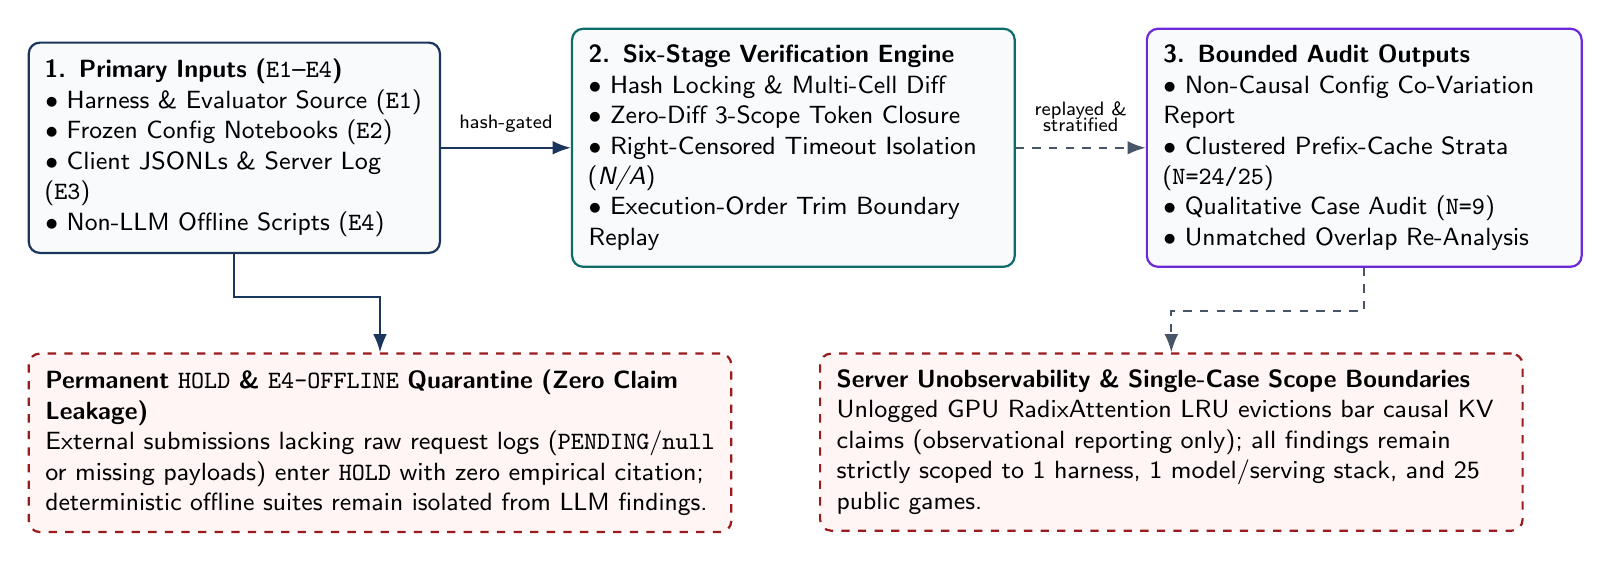
\begin{tikzpicture}[
    font=\sffamily\small,
    stagebox/.style={draw=#1, thick, rounded corners=4pt, fill=bgsoft, inner sep=6pt, align=left, minimum height=2.65cm},
    quarantine/.style={draw=alertred, thick, dashed, rounded corners=4pt, fill=red!4, inner sep=6pt, align=left, minimum height=2.05cm},
    flowarrow/.style={->, >=Latex, thick, draw=navy},
    obsarrow/.style={->, >=Latex, thick, dashed, draw=slate}
]
\node[stagebox=navy, text width=4.8cm] (s1) {
    \textbf{1. Primary Inputs (\code{E1}--\code{E4})}\\
    $\bullet$ Harness \& Evaluator Source (\code{E1})\\
    $\bullet$ Frozen Config Notebooks (\code{E2})\\
    $\bullet$ Client JSONLs \& Server Log (\code{E3})\\
    $\bullet$ Non-LLM Offline Scripts (\code{E4})
};
\node[stagebox=tealdark, text width=5.2cm, right=1.65cm of s1] (s2) {
    \textbf{2. Six-Stage Verification Engine}\\
    $\bullet$ Hash Locking \& Multi-Cell Diff\\
    $\bullet$ Zero-Diff 3-Scope Token Closure\\
    $\bullet$ Right-Censored Timeout Isolation (\na{})\\
    $\bullet$ Execution-Order Trim Boundary Replay
};
\node[stagebox=accentpurple, text width=5.1cm, right=1.65cm of s2] (s3) {
    \textbf{3. Bounded Audit Outputs}\\
    $\bullet$ Non-Causal Config Co-Variation Report\\
    $\bullet$ Clustered Prefix-Cache Strata (\code{N=24/25})\\
    $\bullet$ Qualitative Case Audit (\code{N=9})\\
    $\bullet$ Unmatched Overlap Re-Analysis
};
\node[quarantine, text width=8.5cm, align=left, below=1.25cm of s1.south west, anchor=north west] (q1) {\raggedright
    \textbf{Permanent \code{HOLD} \& \code{E4-OFFLINE} Quarantine (Zero Claim Leakage)}\\
    External submissions lacking raw request logs (\code{PENDING}/\code{null} or missing payloads) enter \code{HOLD} with zero empirical citation; deterministic offline suites remain isolated from LLM findings.
};
\node[quarantine, text width=8.5cm, align=left, right=1.1cm of q1.north east, anchor=north west] (q2) {\raggedright
    \textbf{Server Unobservability \& Single-Case Scope Boundaries}\\
    Unlogged GPU RadixAttention LRU evictions bar causal KV claims (observational reporting only); all findings remain strictly scoped to 1 harness, 1 model/serving stack, and 25 public games.
};
\draw[flowarrow] (s1) -- node[midway, above=2pt, align=center, font=\scriptsize\sffamily] {hash-gated} (s2);
\draw[obsarrow] (s2) -- node[midway, above=2pt, align=center, font=\scriptsize\sffamily] {replayed \&\\[-2pt]stratified} (s3);
\draw[flowarrow] (s1.south) -- ++(0,-0.55) -| (q1.north);
\draw[obsarrow] (s3.south) -- ++(0,-0.55) -| (q2.north);
\end{tikzpicture}%
}
\caption{\textbf{Conceptual Overview of the Evidence-Gated Telemetry Auditing Pipeline.} Solid arrows represent deterministic verification and quarantine routing across local evidence tiers (\code{E1}--\code{E4}); dashed arrows trace execution-order replay and observational stratification explicitly bounded by server-side unobservability and single-case scope.}
\label{fig:pipeline}
\end{figure*}

% ============================================================================
\section{Background, System Under Audit, and Evidence-Gated Protocol}
\label{sec:background}

Before examining configuration drift or token ledgers, we first establish the two prerequisites a reader needs to follow every subsequent result: (1) how an interactive ARC-AGI-3 turn unfolds inside Project HINAGI, and (2) how our Evidence Gate converts heterogeneous artifacts into enforceable claim boundaries.

\subsection{Interactive ARC-AGI-3 Environment and RHAE Intuition}
ARC-AGI-3 \citep{chollet2026arc3} replaces the static input--output pairs of earlier ARC benchmarks with multi-level interactive 2D grid environments. Each game comprises $L$ sequential levels whose hidden transition rules are never revealed in text instructions; an agent discovers mechanics through trial actions (\code{UP}, \code{DOWN}, \code{LEFT}, \code{RIGHT}, \code{SPACE}, coordinate \code{MOUSE(row,col)}). At each physical environment action, the simulator returns the updated grid and two essential signals that we define upfront for use throughout this paper:
\begin{itemize}[leftmargin=1.4em,itemsep=2pt]
\item \textbf{Board-Transition Indicator (\code{bT} vs.\ \code{bF}):} Every executed action triggers either an observable grid change (\code{board\_changed=True}, denoted \code{bT}) or a stagnant no-op / wall-collision transition leaving the board identical (\code{board\_changed=False}, denoted \code{bF}).
\item \textbf{Relative Human Action Efficiency (RHAE):} Mirroring the official \code{EnvironmentScoreCalculator} (v0.9.8) implemented in \code{taaf/game.py:381--413}, RHAE compares the agent's action count $a_l$ on completed level $l \in \{1,\dots,L\}$ against a human baseline $b_l$ (with linear level weights $w_l = l$), combining a \textbf{115\% (1.15) per-level efficiency cap} with a \textbf{100\% (1.00) weighted completion ceiling}:
\end{itemize}
\begin{equation}
\begin{aligned}
s_l &= \min\!\left(115.0,\; 100 \times \left(\frac{b_l}{a_l}\right)^{\!2}\right)\mathbb{I}[\text{completed}_l \land a_l \ge 1], \\
S_{\text{game}} &= \min\!\left(\frac{\sum_{l=1}^L w_l s_l}{\sum_{l=1}^L w_l},\; 100 \times \frac{\sum_{l:\,s_l > 0} w_l}{\sum_{l=1}^L w_l}\right).
\end{aligned}
\label{eq:rhae}
\end{equation}

\begin{conceptbox}{Worked Numerical Example: Why RHAE Penalizes Both Slow Solves and Partial Progress}
Suppose Level~1 has human baseline $b_1 = 10$ actions. If an agent solves Level~1 in $10$ actions, $(10/10)^2 \times 100 = 100.0$. If the agent needs $14$ actions ($40\%$ slower), quadratic scaling slashes the score nearly in half to $100 \times (10/14)^2 = 51.02$. At $20$ actions, efficiency falls to $25.00$. Most critically, because $\mathbb{I}[\text{completed}_l]$ gates every level, failing to finish Level~1 yields $s_1 = 0.0$ regardless of how coherent earlier exploratory moves were---producing the pronounced zero-score floor observed on incomplete runs. Note also the dual caps audited directly in \code{taaf/game.py}: superhuman efficiency on one level saturates at $s_l \le 115.0$, while the game-level completion factor caps $S_{\text{game}}$ at $100 \times (\text{completed weights} / \text{total weights})$.
\end{conceptbox}

\subsection{Project HINAGI Dual-Loop Runtime Architecture}
Project HINAGI executes multi-turn episodes across the 25-game Public Evaluation Split using quantized \textbf{\code{Qwen3.8-Flash-Next}} (W4A16 AutoRound; built on the \code{Qwen3.8-Next} hybrid-reasoning architecture \citep{qiu2026qwen38}) served over HTTP via SGLang \code{0.5.19+gd00d88efc8d6} (\code{pennyroyal-v253} configuration \citep{pezzulli2026pennyroyal}). As shown in Figure~\ref{fig:turn_anatomy}, each episode alternates between an \textbf{outer environment loop} managed by \code{solver.py} / \code{taaf/game.py} and an \textbf{inner reasoning-and-tool loop} inside \code{inference/agent/tool\_agent.py}:
\begin{enumerate}[leftmargin=1.4em,itemsep=2pt]
\item At turn $t$, \code{taaf/game.py} renders the current discrete board as a raster PNG frame (\code{640x640} upscaled grid costing \code{400} payload patch tokens---or \code{402} in the raw PNG sentinel estimate inside \code{\_image\_part\_tokens}, \code{tool\_agent.py:2954--2972}; logged payload frames average \code{400} tokens per inline frame).
\item \code{tool\_agent.py} appends the opener message (board frame + optional state diff image) onto its persistent history and submits an OpenAI-compatible HTTP chat request to SGLang, emitting telemetry into a per-game client log (\code{*\_p0\_requests.jsonl}), an event stream (\code{*\_p0\_events.jsonl}), and server-side \code{ReqTimeStats} rows in \code{serve.log}.
\item Up to \code{TOOL\_STEPS} iterations per turn, the model may generate hidden chain-of-thought reasoning and invoke \code{python\_tool\_sandbox.py} to inspect arrays, test hypotheses, or update persistent workspace variables. When it finally emits a discrete game action (after deterministic pre-dispatch safety guards), the outer loop advances the game state and records token summaries in \code{summary.txt} and \code{benchmark.json}.
\end{enumerate}

\begin{figure}[t]
\centering
\resizebox{0.96\textwidth}{!}{%
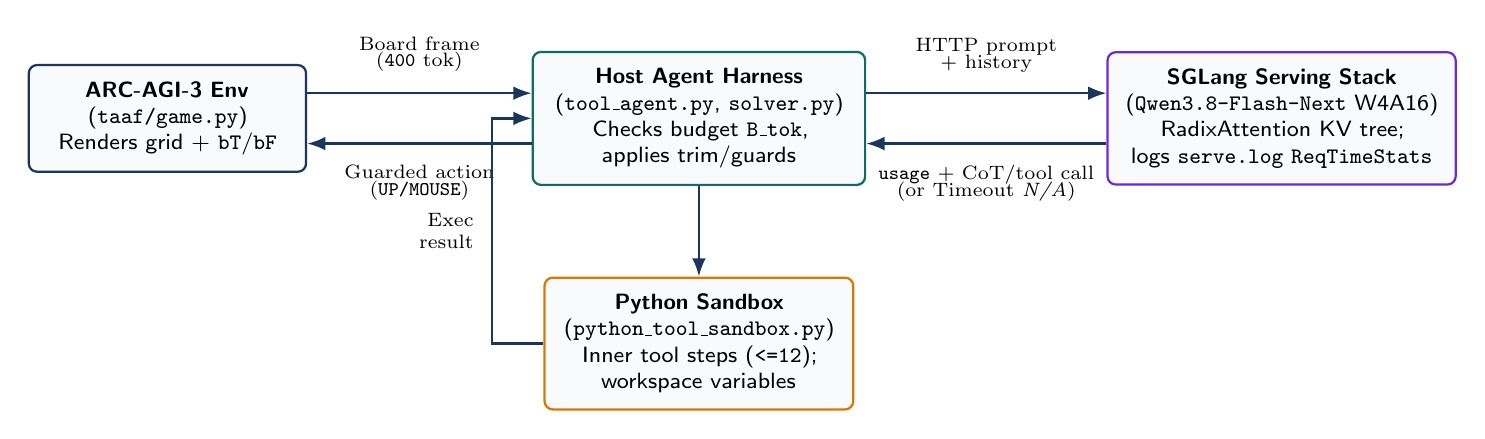
\begin{tikzpicture}[
    font=\sffamily\footnotesize,
    box/.style={draw=#1, thick, rounded corners=3pt, fill=bgsoft, inner sep=6pt, align=center},
    arrow/.style={->, >=Latex, thick, draw=navy}
]
\node[box=navy, text width=3.1cm] (env) {\textbf{ARC-AGI-3 Env}\\(\code{taaf/game.py})\\Renders grid + \code{bT}/\code{bF}};
\node[box=tealdark, text width=3.8cm, right=2.85cm of env] (host) {\textbf{Host Agent Harness}\\(\code{tool\_agent.py}, \code{solver.py})\\Checks budget \code{B\_tok}, applies trim/guards};
\node[box=accentorange, text width=3.5cm, below=1.15cm of host] (sbx) {\textbf{Python Sandbox}\\(\code{python\_tool\_sandbox.py})\\Inner tool steps (\code{<=12});\\workspace variables};
\node[box=accentpurple, text width=4.0cm, right=3.05cm of host] (srv) {\textbf{SGLang Serving Stack}\\(\code{Qwen3.8-Flash-Next} W4A16)\\RadixAttention KV tree;\\logs \code{serve.log} \code{ReqTimeStats}};
\draw[arrow] ([yshift=0.32cm]env.east) -- node[above=4pt, align=center, font=\scriptsize] {Board frame\\[-2pt](\code{400} tok)} ([yshift=0.32cm]host.west);
\draw[arrow] ([yshift=-0.32cm]host.west) -- node[below=4pt, align=center, font=\scriptsize] {Guarded action\\[-2pt](\code{UP/MOUSE})} ([yshift=-0.32cm]env.east);
\draw[arrow] (host.south) -- (sbx.north);
\draw[arrow] (sbx.west) -- ++(-0.65,0) |- node[left=3pt, pos=0.25, font=\scriptsize, align=right] {Exec\\result} (host.west);
\draw[arrow] ([yshift=0.32cm]host.east) -- node[above=4pt, align=center, font=\scriptsize] {HTTP prompt\\[-2pt]+ history} ([yshift=0.32cm]srv.west);
\draw[arrow] ([yshift=-0.32cm]srv.west) -- node[below=4pt, align=center, font=\scriptsize] {\code{usage} + CoT/tool call\\[-2pt](or Timeout \na{})} ([yshift=-0.32cm]host.east);
\end{tikzpicture}%
}
\caption{\textbf{Anatomy of a Single Interactive Turn in Project HINAGI.} One outer environment action can span multiple HTTP requests (via inner Python sandbox steps), illustrating how action-attributed summaries capture only a subset of client completions and why client/server boundaries require explicit reconciliation.}
\label{fig:turn_anatomy}
\end{figure}

Table~\ref{tab:provenance} inventories every verified primary artifact, its SHA-256 digest on disk, and its functional role in this audit.

\begin{table*}[t]
\centering
\caption{\textbf{Verified Primary Source, Configuration, and Local Log Provenance (\code{E1}--\code{E3}, Verification Suite, \& External Reference).}}
\label{tab:provenance}
\resizebox{\textwidth}{!}{%
\begin{tabular}{@{}lll>{\raggedright\arraybackslash}p{6.5cm}@{}}
\toprule
\textbf{Tier} & \textbf{Artifact (Repo-Relative Path)} & \textbf{SHA-256 Prefix / Full Digest} & \textbf{Role / Audited Scope} \\
\midrule
\code{E1} & \code{reference/.../agent/tool\_agent.py} & \code{053556f4a2d19bbb} & Calibration clamping (\code{[1.0, 3.3]}), budget \code{B\_tok=44,544}, trim execution (\code{L6323, L6699, L7184}) \\
\code{E1} & \code{reference/.../framework/solver.py} & \code{42b4794f0447e071} & Wallclock \code{started\_at} init (\code{L480}), runtime polling (\code{L522, L624}), \code{solver\_note} (\code{L1252}) \\
\code{E1} & \code{reference/.../python\_tool\_sandbox.py} & \code{3900b7255842df04} & Pre-dispatch host safety checks \& \code{KnownDeathActionError} (\code{L420--711}) \\
\code{E1} & \code{reference/.../src/taaf/game.py} & \code{8609e0646e96616d} & Official RHAE calculation (\code{115\%} level cap, \code{100\%} game cap, \code{L381--413}) \\
\code{E2} & \code{artifacts/phase6\_5/.../v6\_reference.ipynb} & \parbox[t]{5.85cm}{\raggedright\code{bb532e8c502ac5ce72c36918a2b1ac90\allowbreak e0de3cc96f5bdc70682953914466c90e}} & V6 23-cell baseline notebook (\code{18/23} cells byte-identical to V10) \\
\code{E2} & \code{artifacts/phase6\_5/.../v10\_reference.ipynb} & \code{5f940b9615dee4ab} & V10 23-cell notebook (\code{Cells \{0,4,6,12,16\}} modified; \code{Cell 2} \code{498,799} chars) \\
\code{E3} & \code{submissions/arc3\_v10\_verified/benchmark.json} & \code{8ee5206704b21d4e} & Canonical 25-game V10 scores (\code{sum = 70.937500}), \code{started\_at}, physical actions \\
\code{E3} & \code{submissions/arc3\_v10\_verified/summary.txt} & \code{878381b48014433b} & CLI action summary (\code{378,304} action-attributed tokens, \code{386} physical actions) \\
\code{E3} & \code{submissions/arc3\_v10\_verified/requests.jsonl} & \code{c3d3e9e5ecee90d8} & Root fallback client log containing detached \code{g50t c\_idx=15} (\code{+2,778} tok) \\
\code{E3} & \code{submissions/arc3\_v10\_verified/serve.log} & \code{755a22bd7f41e1a8} & SGLang server log (\code{360} \code{ReqTimeStats}, first \code{/health 200 OK} \code{05:15:53}, \code{4} timeout tails) \\
\code{E3} & \code{submissions/arc3\_v6\_smoke\_verified/benchmark.json} & \code{1f9975ef4d29a6e5} & Unmatched 25-game V6 smoke baseline (\code{10/25} active, \code{15/25} starved; JSONLs absent) \\
\code{R1} & \code{HINAGI\_R3\_2\_PUBLIC\_RELEASE/} & \code{f0eee5579910df73} & Clean-room deterministic CPU replay suite (\code{141/141} public; \code{140/140} Original R1) \\
\bottomrule
\end{tabular}%
}
\end{table*}

\subsection{Operational Evidence Gate (\code{E1}--\code{E4}) vs.\ Permanent \code{HOLD} Quarantine}
Think of this taxonomy like an aviation safety investigation: verified flight-recorder telemetry (\code{E3}), cockpit design specifications (\code{E1}--\code{E2}), and isolated bench simulations (\code{E4}) form graded evidentiary layers, whereas an unrecovered external log tape (\code{HOLD}) is \emph{not} a weaker fifth tier---it is a \textbf{zero-citation sealed locker} that cannot be averaged into or guessed alongside observed data. Algorithm~1 specifies the complete 6-stage procedure so any independent auditor can execute the exact same pipeline, and Table~\ref{tab:protocol_schema} maps allowed versus prohibited claim structures.

\begin{figure}[t]
\centering
\begin{conceptbox}{Algorithm 1: Operational Six-Stage Evidence-Gated Telemetry Auditing Procedure}
\textbf{Stage 1 (Provenance Locking):} Compute SHA-256 checksums across all source, notebook, log, and summary files.\\
\textbf{Stage 2 (Quarantine Classification):} Route any external ID missing raw request/response payloads or carrying \code{PENDING/null} status into permanent \code{HOLD}; route deterministic zero-LLM scripts into \code{E4-OFFLINE}.\\
\textbf{Stage 3 (Multi-Cell Configuration Audit):} Diff full launch notebooks cell-by-cell; if $|{\Delta\text{cells}}| > 1$, lock cross-run comparisons as confounded and unmatched. Cross-check prose markdown headers directly against code and timestamps.\\
\textbf{Stage 4 (Three-Scope Zero-Imputation Closure):} Reconcile action-history totals ($S_1$), per-game JSONL completions ($S_2$), and root-fallback records ($S_3$) to machine zero against \code{solver\_note} sums. Classify client HTTP read timeouts strictly as right-censored \na{}; inspect \code{serve.log} separately without adding server \code{output\_len} into client totals.\\
\textbf{Stage 5 (Execution-Order Boundary Replay):} Deduplicate calibration emissions by \code{(timestamp, step, ratio)}, then step through runtime message assembly in exact source order to capture both turn-end and next-opener trim checkpoints.\\
\textbf{Stage 6 (Clustered Stratification \& Observational Bounds):} Stratify prefix transitions by host message-array diffs, report token-weighted pooled alongside game-cluster means ($N$), and withhold GPU causal claims whenever server LRU eviction events go unlogged.
\end{conceptbox}
\end{figure}

\begin{table*}[t]
\centering
\caption{\textbf{Four Local Evidence Tiers vs.\ \code{HOLD} Quarantine Definition, Primary Schema Keys, and Claim-Boundary Rules.}}
\label{tab:protocol_schema}
\resizebox{\textwidth}{!}{%
\begin{tabular}{@{}l >{\raggedright\arraybackslash}p{4.1cm} >{\raggedright\arraybackslash}p{5.3cm} >{\raggedright\arraybackslash}p{5.3cm}@{}}
\toprule
\textbf{Category} & \textbf{Schema / Primary Keys Verified} & \textbf{Allowed Claim Example (Bounded)} & \textbf{Prohibited Claim (Blocked by Protocol)} \\
\midrule
\code{E1-SOURCE} & Algorithm constants, \code{B\_tok}, \code{\_calibrate\_\allowbreak from\_usage}, RHAE \code{taaf/game.py} & ``Client budget computes \code{44,544} tokens via 56K$-$12K$-$512 with \code{[1.0, 3.3]} clamping.'' & ``Clamping improved solver accuracy across unobserved competition runs.'' \\
\code{E2-CONFIG} & 23-cell notebook diffs (\code{Cell 0, 4, 6, 12, 16}), env vars, \code{started\_at} reset & ``Five cells changed concurrently between V6 and V10; Cell~0 contradicts Cell~6 delay.'' & ``Modifying \code{Cell 16} or \code{DRAIN=16K} independently caused V10's higher score.'' \\
\code{E3-LOCAL-LOG} & \code{*\_p0\_requests.jsonl} (\code{usage}), root \code{requests.jsonl}, \code{events}, \code{serve.log} & ``Client completions close exactly (\code{471,288, diff=0}) across 25 games; 4 timeouts stay \na{}.'' & ``Mutations caused GPU LRU eviction (\code{p < 0.001} over \code{n=69} i.i.d.\ requests).'' \\
\code{E4-OFFLINE} & Zero-LLM scripts (\code{Phase 6.0}, \code{matched\_\allowbreak evaluation\_\allowbreak results.json}) & ``Offline replay hits \code{260.40} across 25 games / 39 levels in \code{1.42s} with 0 LLM calls.'' & ``Phase~6.0 proves a controlled $2\times 2$ LLM ablation (retracted from v6.4).'' \\
\textbf{\code{HOLD}} & Missing payloads (\code{57758308}, \code{57827259 PENDING/null}, \code{57912660}) & ``Three hosted Kaggle submissions lack raw request logs and remain permanently quarantined.'' & ``V10 scored 8.03 vs.\ V6 33.38 on private Kaggle evaluations.'' \\
\bottomrule
\end{tabular}%
}
\end{table*}

% ============================================================================
\section{Configuration Co-Variation Audit: Why V6 vs.\ V10 Is Not a Controlled Ablation}
\label{sec:config}

Before inspecting any token sum or score, an auditor must ask: \emph{Are \code{V6} and \code{V10} a clean one-factor ablation where only context budget changed, or a multi-variable system overhaul?} Comparing all 23 cells of \code{v6\_reference.ipynb} and \code{v10\_reference.ipynb} proves that \code{18} cells---including the \code{498,799}-character \code{Cell 2} core engine---are byte-identical, while \textbf{\code{5} cells (\code{Cells 0, 4, 6, 12, 16}) co-varied simultaneously} (Table~\ref{tab:notebookdiff}).

\subsection{Plain-English Guide to Co-Varying Parameters (\code{Cell 4} \& \code{Cell 12})}
Like changing oven temperature, flour ratio, and baking time simultaneously in a single recipe test, co-varying knobs make single-factor causal attribution impossible:
\begin{itemize}[leftmargin=1.4em,itemsep=2pt]
\item \textbf{Context Window \& Drain (\code{128K / 58K} $\to$ \code{56K / 16K}):} \code{V10} halves the budget to \code{(44+12)*1024 = 57,344} (\code{B\_tok = 44,544} input cap), turning on aggressive pruning whenever prompts expand, and sets the drain target (\code{ARC3\_CONTEXT\_DRAIN\_TOKENS}) to \code{16K}, dropping target occupancy down to \code{44,544 - 16,384 = 28,160} tokens upon FIFO eviction.
\item \textbf{Inner Sandbox Loops (\code{TOOL\_STEPS=0} $\to$ \code{12}) \& Turn Limit (\code{150} $\to$ \code{36}):} Enabling 12 Python sandbox calls per game step lets the agent analyze grids deeply per turn, shrinking max outer turns from 150 to 36 while dramatically inflating per-turn reasoning tokens.
\item \textbf{In-Place Image Window (\code{IMAGE\_KEEP=4}) \& Control Pruning (\code{PRUNE\_CONTROL=1}):} \code{IMAGE\_KEEP=4} replaces older inline board frames with text placeholders once more than 4 historical frames accumulate, while \code{PRUNE\_CONTROL=1} drops duplicate yield-resumption prompts. \code{WM\_WIPE=0} disables clearing the agent's working-memory counter on trim.
\item \textbf{Model Pre-caching \& OS Page Cache (\code{Cell 6} \& \code{Cell 12}):} Changing \code{precache\_model\_thread} delay (\code{60s} $\to$ \code{30s}) and \code{DROP\_CACHE\_AFTER\_LOAD} (\code{True} $\to$ \code{False}) alters disk I/O contention during server startup alongside sampling temperature (\code{0.7} $\to$ \code{0.6}) and memory section verbosity (\code{off} $\to$ \code{medium}).
\end{itemize}

\begin{table*}[t]
\centering
\caption{\textbf{Concurrent Configuration Changes Between \code{v6\_reference.ipynb} and \code{v10\_reference.ipynb} (\code{5/23} Cells) and Audit Verdicts.}}
\label{tab:notebookdiff}
\resizebox{\textwidth}{!}{%
\begin{tabular}{@{}l >{\raggedright\arraybackslash}p{4.1cm} >{\raggedright\arraybackslash}p{4.7cm} >{\raggedright\arraybackslash}p{4.6cm}@{}}
\toprule
\textbf{Cell} & \textbf{V6 Smoke Baseline} & \textbf{V10 Audited Configuration} & \textbf{Audit Verdict / Co-Variation Implication} \\
\midrule
\code{Cell 0} & Architecture 3.0 prose header & Claims zero I/O contention ($\sim$340\,s boot), ``guarantee zero Read timed out'', and \code{18K} handover & \textbf{3 Prose Claims Falsified:} \code{Cell 6} retains \code{precache\_\allowbreak model\_thread}; \code{4} HTTP timeouts occur; \code{0} handover tokens emitted \\
\code{Cell 4} & \code{CONTEXT=128K}, \code{DRAIN=58K}, \code{TURNS=150}, \code{TOOL\_\allowbreak STEPS=0}, \code{TEMP=0.7}, \code{MEMORY=off}, \code{6} guards & \code{CONTEXT=(44+12)K} (\code{B\_tok=44,544}), \code{DRAIN=16K}, \code{TURNS=36}, \code{TOOL\_\allowbreak STEPS=12}, \code{TEMP=0.6}, \code{MEMORY=medium}, \code{7} guards & \textbf{Confounded Co-Variation:} Tighter budget enabled trims alongside \code{IMAGE\_KEEP=4}, \code{PRUNE\_\allowbreak CONTROL=1}, \code{WM\_WIPE=0} \\
\code{Cell 6} & \code{precache\_\allowbreak model\_\allowbreak thread(..., delay=60)} & \code{precache\_\allowbreak model\_\allowbreak thread(..., delay=30)} & Contradicts Cell~0 claim of disabled I/O contention thread \\
\code{Cell 12} & \code{DROP\_CACHE\_\allowbreak AFTER\_LOAD=True} & \code{DROP\_CACHE\_\allowbreak AFTER\_LOAD=False} & Alters OS page cache concurrently with server warm-up \\
\code{Cell 16} & Static setup; \code{max\_runtime=600.0s}; no \code{/health} wait or timer reset & Adds \code{/health} poll + \code{self.started\_at = time.monotonic()} reset, \code{max(30.0, t)}, \code{15s} stop margin, \code{18K} quantum flag & \textbf{Identical \code{600.0s} Cap; Concurrency Shift:} Excludes $\sim$496\,s server boot from game clock (\code{05:07:36} init vs.\ \code{05:15:53} ready) \\
\bottomrule
\end{tabular}%
}
\end{table*}

\subsection{Falsified Notebook Claims \& The Wallclock Boot-Reset Mechanism}
Two findings from Table~\ref{tab:notebookdiff} reshape how \code{V6} and \code{V10} must be interpreted:
\begin{enumerate}[leftmargin=1.4em,itemsep=2pt]
\item \textbf{Three Falsified Prose Assertions (\code{Cell 0}):} First, \code{Cell 0} promises zero background I/O contention by disabling model precaching, yet \code{Cell 6} still launches \code{precache\_model\_thread(..., delay=30)}. Second, \code{Cell 0} guarantees zero HTTP read timeouts, yet \code{serve.log} and client logs document \code{4} client read timeouts (\code{30.00s}--\code{50.92s}). Third, \code{Cell 0} and \code{Cell 16} advertise an \code{18K} quantum context handover mechanism, yet client logs verify \code{0} handover summary tokens generated anywhere across the 25 games.
\item \textbf{Wallclock Reset Mechanism (\code{Cell 16}, Figure~\ref{fig:wallclock}):} Imagine starting a 600-second exam stopwatch while the printing press is still warming up for 496 seconds versus resetting the stopwatch once papers reach desks. Both \code{V6} and \code{V10} configure \code{bm.solver.max\_runtime\_s\_per\_game = 600.0}. In \code{V10}, \code{benchmark.json} records initial \code{started\_at} between \code{05:07:36.57} and \code{05:07:38.06}, whereas \code{serve.log} logs its first \code{GET /health 200 OK} only at \code{05:15:53} ($\sim$496\,s later). Because \code{V10 Cell 16} polls \code{/health} and overwrites \code{self.started\_at = time.monotonic()} afterward (\code{solver.py:480, 522, 624}), \code{V10} games ran \code{1089.88}--\code{1361.82s} total wallclock (\code{25/25} active streams) rather than expiring at \code{600.18}--\code{605.99s} (\code{15/25} starved streams with \code{0} actions) as in \code{V6}. Because \code{Cells 4, 6, 12, 16} co-varied and \code{V6} lacks JSONL request logs, we characterize this strictly as a structural mechanism without claiming single-cell causal score attribution.
\end{enumerate}

\begin{figure}[t]
\centering
\resizebox{0.96\textwidth}{!}{%
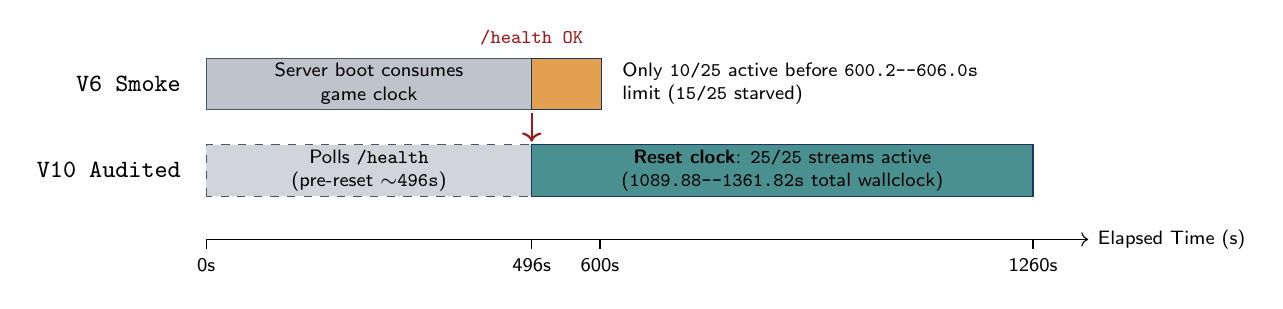
\begin{tikzpicture}[font=\sffamily\footnotesize]
\draw[->] (0,0) -- (11.2,0) node[right] {\scriptsize Elapsed Time (s)};
\foreach \x/\lbl in {0/0s, 4.133/496s, 5.0/600s, 10.5/1260s} {
    \draw (\x,0) -- (\x,-0.12) node[below] {\scriptsize \lbl};
}
% V6 row (scale: 1cm = 120s)
\node[anchor=east, font=\sffamily\small\bfseries] at (-0.2,1.98) {\code{V6 Smoke}};
\fill[slate!35, draw=slate] (0,1.65) rectangle (4.133,2.30);
\node[align=center] at (2.067,1.975) {\scriptsize Server boot consumes\\[-1pt]\scriptsize game clock};
\fill[accentorange!70, draw=navy] (4.133,1.65) rectangle (5.017,2.30);
\node[anchor=west, align=left] at (5.16,1.975) {\scriptsize Only \code{10/25} active before \code{600.2--606.0s}\\[-1pt]\scriptsize limit (\code{15/25} starved)};
% V10 row
\node[anchor=east, font=\sffamily\small\bfseries] at (-0.2,0.88) {\code{V10 Audited}};
\fill[slate!25, draw=slate, dashed] (0,0.55) rectangle (4.133,1.20);
\node[align=center] at (2.067,0.875) {\scriptsize Polls \code{/health}\\[-1pt]\scriptsize (pre-reset \code{$\sim$496s})};
\fill[tealdark!75, draw=navy] (4.133,0.55) rectangle (10.5,1.20);
\node[align=center] at (7.317,0.875) {\scriptsize \textbf{Reset clock}: \code{25/25} streams active\\[-1pt]\scriptsize (\code{1089.88--1361.82s} total wallclock)};
\draw[alertred, thick, ->] (4.133,1.60) -- (4.133,1.24);
\node[anchor=south, text=alertred, font=\scriptsize, inner sep=1pt] at (4.133,2.42) {\code{/health OK}};
\end{tikzpicture}%
}
\caption{\textbf{Boot-Latency Exclusion and Concurrency Shift Between \code{V6} and \code{V10}.} Both runs retain \code{max\_runtime\_s\_per\_game = 600.0}. Polling \code{/health} before resetting \code{self.started\_at} activated all \code{25} streams in \code{V10}, whereas \code{15/25} queued streams starved with \code{0} actions in \code{V6}.}
\label{fig:wallclock}
\end{figure}

\subsection{Host Safety Guards Without Counterfactuals (\code{17/386} Overall \code{bF})}
Informal project notes occasionally attributed \code{V10}'s behavior to newly added safety checks. Static diffing (\code{E1}/\code{E2}, \code{python\_\allowbreak tool\_\allowbreak sandbox.py:420--711}) disproves that view: \code{V6 Cell 4} already enabled six deterministic pre-dispatch checks (\code{ARC3\_BATCH\_\allowbreak NOOP\_BLOCK}, \code{ARC3\_STALE\_\allowbreak STATE\_BLOCK}, \code{ARC3\_REPEAT\_\allowbreak STATE\_GUARD}, \code{ARC3\_DEATH\_\allowbreak REPEAT\_GUARD}, \code{ARC3\_DEATH\_\allowbreak GUARD\_\allowbreak LOOKAHEAD}, \code{ARC3\_BOARD\_\allowbreak DUMP\_GUARD}), grouped functionally into (a) no-op/stale-state blocking, (b) known-death/repeat-loop blocking (\code{KnownDeathActionError}), and (c) redundant board-dump suppression. \code{V10} kept all six and added \code{ARC3\_NOOP\_\allowbreak REPEAT\_GUARD='1'}. Across \code{V10}'s \code{386} executed physical actions, stagnant \code{bF} transitions occurred \code{17/386} times (\code{4.40\%}). Crucially, because the harness neither logged rejected-candidate action counters nor ran a \code{Guard-OFF} counterfactual control, we report \code{17/386} strictly as an observed post-guard rate without claiming empirical guard effectiveness.

% ============================================================================
\section{Three-Scope Client Token Reconciliation and Timeout Forensics}
\label{sec:accounting}

\subsection{Lifecycle of a Request: Why Three Accounting Scopes Disagree}
Auditors often expect a single run to yield a single token total, yet parsing \code{summary.txt}, per-game JSONLs, and \code{benchmark.json} produces three distinct numbers (\code{378,304}, \code{468,510}, \code{471,288}). Consider an analogy to household expense ledgers: (1) receipts for ingredients actually cooked into dinner (\textbf{Scope 1}); (2) receipts sitting on the kitchen counter including unfinished snacks (\textbf{Scope 2}); and (3) one loose receipt accidentally dropped on the hallway table (\textbf{Scope 3}), while four deliveries hung up mid-order (\textbf{Right-Censored \code{N/A}}). Tracing the actual software pipeline resolves all three figures to zero error (\code{diff = 0}, Figure~\ref{fig:request_lifecycle}, Table~\ref{tab:tokens}):
\begin{enumerate}[leftmargin=1.4em,itemsep=2pt]
\item \textbf{Scope 1 --- Action-Attributed History (\code{378,304} tokens):} Both \code{summary.txt} and \code{benchmark.json} (\code{history\_generated\_tokens}) sum completion tokens \emph{only} for inference chains culminating in one of the \code{386} executed physical actions, ignoring trailing non-action turns.
\item \textbf{Scope 2 --- Per-Game Request Logs (\code{468,510} tokens, \code{352} responses):} Summing \code{usage.\allowbreak completion\_\allowbreak tokens} over all 25 per-game \code{*\_p0\_\allowbreak requests.\allowbreak jsonl} logs covers \code{357} client requests and \code{352} delivered responses (\code{404,005} reasoning = \code{86.23\%}; \code{7,078,878} prompt; \code{4,480,704} cached = \code{63.30\%}), leaving \code{90,206} valid trailing non-action tokens (\code{19.25\%}).
\item \textbf{Scope 3 --- Full Client Delivered Responses (\code{471,288 == sum(solver\_note)}, \code{353} responses):} One HTTP response in game \code{g50t-5849a774} (\code{c\_idx=15}: \code{19,438} prompt, \code{16,064} cached, \code{2,778} completion, \code{2,391} reasoning) lost its per-game logger binding and fell back to the shared root \code{requests.jsonl}. Adding that single delivered record closes Scope~2 $\to$ Scope~3 (\code{468,510 + 2,778 = 471,288}; \code{406,396} reasoning = \code{86.23\%}; \code{7,098,316} prompt; \code{4,496,768} cached = \code{63.35\%}), matching \code{benchmark.json} \code{solver\_note} (\code{solver.py:1252}) with \textbf{\code{0}-token discrepancy across all \code{25/25} games} (\code{Comp\_353 = ActTok + Trail\_353}, where \code{Trail\_353 = 92,984}). Meanwhile, \code{0} handover summary tokens were emitted anywhere.
\end{enumerate}

\begin{figure}[t]
\centering
\resizebox{0.96\textwidth}{!}{%
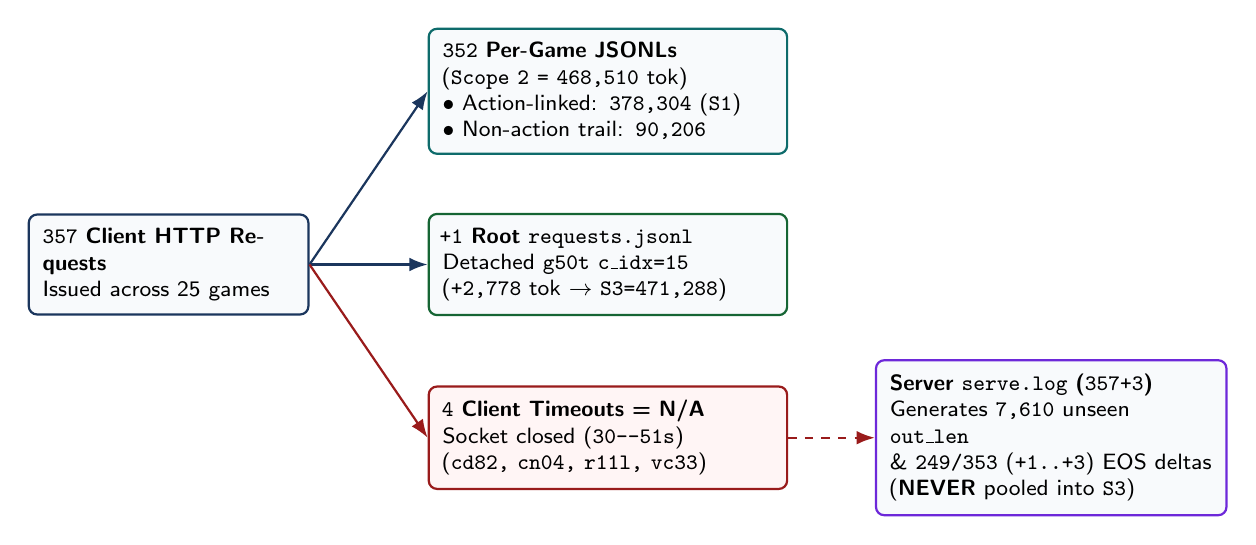
\begin{tikzpicture}[
    font=\sffamily\footnotesize,
    pnode/.style={draw=#1, thick, rounded corners=3pt, fill=bgsoft, inner sep=5pt, align=left},
    arrow/.style={->, >=Latex, thick, draw=navy}
]
\node[pnode=navy, text width=3.2cm] (reqs) {\textbf{\code{357} Client HTTP Requests}\\Issued across 25 games};
\node[pnode=tealdark, text width=4.2cm, right=1.5cm of reqs, yshift=2.20cm] (pg) {\textbf{\code{352} Per-Game JSONLs}\\(\code{Scope 2 = 468,510} tok)\\$\bullet$ Action-linked: \code{378,304} (\code{S1})\\$\bullet$ Non-action trail: \code{90,206}};
\node[pnode=okgreen, text width=4.2cm, right=1.5cm of reqs, yshift=0.0cm] (root) {\textbf{\code{+1} Root \code{requests.jsonl}}\\Detached \code{g50t c\_idx=15}\\(\code{+2,778} tok $\to$ \code{S3=471,288})};
\node[pnode=alertred, fill=red!4, text width=4.2cm, right=1.5cm of reqs, yshift=-2.20cm] (to) {\textbf{\code{4} Client Timeouts = \na{}}\\Socket closed (\code{30--51s})\\(\code{cd82, cn04, r11l, vc33})};
\node[pnode=accentpurple, text width=4.1cm, right=1.1cm of to] (srv) {\textbf{Server \code{serve.log} (\code{357+3})}\\Generates \code{7,610} unseen \code{out\_len}\\\& \code{249/353} (\code{+1..+3}) EOS deltas\\(\textbf{NEVER} pooled into \code{S3})};
\draw[arrow] (reqs.east) -- (pg.west);
\draw[arrow] (reqs.east) -- (root.west);
\draw[arrow, draw=alertred] (reqs.east) -- (to.west);
\draw[->, >=Latex, thick, dashed, draw=alertred] (to.east) -- (srv.west);
\end{tikzpicture}%
}
\caption{\textbf{Routing of All \code{357} Client HTTP Requests Across Client Ledgers and Server Completions.} Recovering the single detached root fallback response (\code{g50t c\_idx=15}) closes client totals to \code{diff=0}, while \code{4} timed-out client calls remain strictly right-censored (\na{}) separate from server-side \code{serve.log} generation.}
\label{fig:request_lifecycle}
\end{figure}

\subsection{No-Imputation Timeout Firewall, Server EOS Drift, and Uncensored Trailing Gaps}
Suppose a 30-second phone call drops mid-sentence: recording "zero words spoken" mistakes signal interruption for silence, yet blindly pasting the speaker's unsent transcript fails if both sides count punctuation differently. Exactly this telemetry mismatch occurs between the agent harness and SGLang in \code{serve.log} (\code{360} \code{ReqTimeStats} records = \code{3} warmups + \code{357} game calls):
\begin{enumerate}[leftmargin=1.4em,itemsep=2pt]
\item On all \code{4} client timeouts (\code{cd82}, \code{cn04}, \code{r11l}, \code{vc33} at \code{serve.log} lines \code{1562, 1723, 1787, 1879}), the GPU worker finished decoding after client socket teardown, producing \textbf{\code{7,610} unreceived server \code{output\_len} tokens} (\code{1,928 + 2,902 + 1,713 + 1,067}).
\item Across the \code{353} \emph{delivered} pairs, server \code{output\_len} exceeds client \code{usage.completion\_tokens} by \code{1}--\code{3} tokens on \textbf{\code{249/353} (\code{70.5\%})} requests (\code{deltas = {0: 104, +1: 56, +2: 111, +3: 82}}), reflecting stop/EOS accounting divergence between server runtime stats and API usage billing.
\end{enumerate}

Therefore, V12 enforces a strict \textbf{No-Imputation Firewall}: the 4 client timeout tails remain \textbf{right-censored \na{}}, never coded as \code{0} and never merged with \code{serve.log}'s \code{7,610} tokens. Inspecting \textbf{uncensored} trailing non-action gaps strictly on complete episodes contrasts \textbf{\code{N=5} uncensored Evicted games} (\code{ar25} \code{1,003}, \code{bp35} \code{7,723}, \code{ft09} \code{1,247}, \code{g50t} \code{5,147} [\code{353}] / \code{2,369} [\code{352}], \code{sb26} \code{807}: \code{mean = 3,185.40}, \code{median = 1,247.0} at \code{353} scope; \code{mean = 2,629.80} at \code{352} scope) against \textbf{\code{N=16} Non-Evicted games} (\code{sum = 63,597}, \code{mean = 3,974.81}, \code{median = 3,450.0}), noting that the case of \code{r11l-495a7899} cleanly illustrates this rule: response \code{c\_idx=12} delivered \code{13,460} non-action trailing tokens cleanly (\code{Comp = 20,168 + 13,460 = 33,628}), after which final request \code{c\_idx=13} timed out at \code{30.00s} (\code{server output\_len=1,713}), placing \code{r11l} conservatively in the censored group (Table~\ref{tab:tokens}; Figure~\ref{fig:tokens}).

\begin{table*}[t]
\centering
\caption{\textbf{Three-Scope Client Token Reconciliation, Right-Censored Timeouts (\na{}), and Uncensored Trailing Gaps (\code{V10}; Identity: \code{Comp\_353 = ActTok + Trail\_353}).}}
\label{tab:tokens}
\resizebox{\textwidth}{!}{%
\setlength{\tabcolsep}{4pt}
\begin{tabular}{@{}l r r r r r r r r l@{}}
\toprule
\textbf{Cohort / Game} & \textbf{Score} & \textbf{Acts} & \textbf{Req/Resp} & \textbf{Prompt\,(353)} & \textbf{Cached\,(353)} & \textbf{ActTok} & \textbf{Comp\,(352/353)} & \textbf{Trail\,(353)} & \textbf{Client Status / Server Note} \\
\midrule
\code{ar25-0c556536} & 8.3333 & 42 & 22 / 22 & 505,315 & 199,488 & 23,453 & 24,456 & 1,003 & graceful (\code{diff=0}) \\
\code{bp35-0a0ad940} & 0.0000 & 8 & 15 / 15 & 365,979 & 309,888 & 12,124 & 19,847 & 7,723 & graceful (\code{diff=0}) \\
\code{cd82-fb555c5d} & 0.0000 & 10 & 15 / 14 & 265,309 & 145,408 & 18,510 & 18,510 & \na{} (TO) & HTTP TO \code{49.14s}; \code{srv\_out=1,928} \\
\code{cn04-2fe56bfb} & 4.7619 & 27 & 14 / 13 & 310,949 & 181,184 & 28,304 & 28,304 & \na{} (TO) & HTTP TO \code{50.92s}; \code{srv\_out=2,902} \\
\code{ft09-0d8bbf25} & 28.5714 & 26 & 14 / 14 & 339,873 & 199,936 & 26,347 & 27,594 & 1,247 & graceful (\code{diff=0}) \\
\code{g50t-5849a774} & 0.0000 & 13 & 16 / 15+1 & 343,711 & 243,584 & 26,532 & 28,901 / 31,679 & 5,147 & \code{+2,778} root \code{c\_idx=15} (\code{352: 2,369}) \\
\code{r11l-495a7899} & 4.7619 & 10 & 14 / 13 & 317,280 & 218,048 & 20,168 & 33,628 & 13,460$^\dagger$ & \code{c\_idx=12} trail \code{13,460}; \code{c\_idx=13} TO \code{30.0s} (\code{srv=1,713})$^\dagger$ \\
\code{sb26-7fbdac44} & 2.7778 & 34 & 24 / 24 & 610,268 & 322,880 & 22,469 & 23,276 & 807 & graceful (\code{diff=0}) \\
\code{vc33-5430563c} & 9.4296 & 34 & 20 / 19 & 407,886 & 205,504 & 25,854 & 25,854 & \na{} (TO) & HTTP TO \code{30.00s}; \code{srv\_out=1,067} \\
\midrule
\textbf{Evicted (\code{N=9})} & \textbf{58.6359} & \textbf{204} & \textbf{154 / 150} & \textbf{3,466,570} & \textbf{2,025,920} & \textbf{203,761} & \textbf{230,370 / 233,148} & \textbf{29,387} & \textbf{Uncensored \code{N=5}: mean \code{3,185.4} (353)} \\
\textbf{Non-Evicted (\code{N=16})} & \textbf{12.3016} & \textbf{182} & \textbf{203 / 203} & \textbf{3,631,746} & \textbf{2,470,848} & \textbf{174,543} & \textbf{238,140 / 238,140} & \textbf{63,597} & \textbf{Uncensored \code{N=16}: mean \code{3,974.8}} \\
\midrule
\textbf{All \code{25} Games} & \textbf{70.9375} & \textbf{386} & \textbf{357 / 353} & \textbf{7,098,316} & \textbf{4,496,768} & \textbf{378,304} & \textbf{468,510 / 471,288} & \textbf{92,984} & \textbf{4 client TO = \na{}; \code{sum(srv)=7,610}} \\
\bottomrule
\end{tabular}%
}
\par\vspace{2pt}
\raggedright\scriptsize{$^\dagger$\code{r11l-495a7899} executed \code{c\_idx=12} (\code{13,460} non-action trailing tokens) before final request \code{c\_idx=13} timed out (\code{30.00s}, server \code{1,713}), so \code{r11l} is conservatively excluded from uncensored \code{N=5} averages.}
\end{table*}

\begin{figure}[t]
\centering
\resizebox{0.96\textwidth}{!}{%
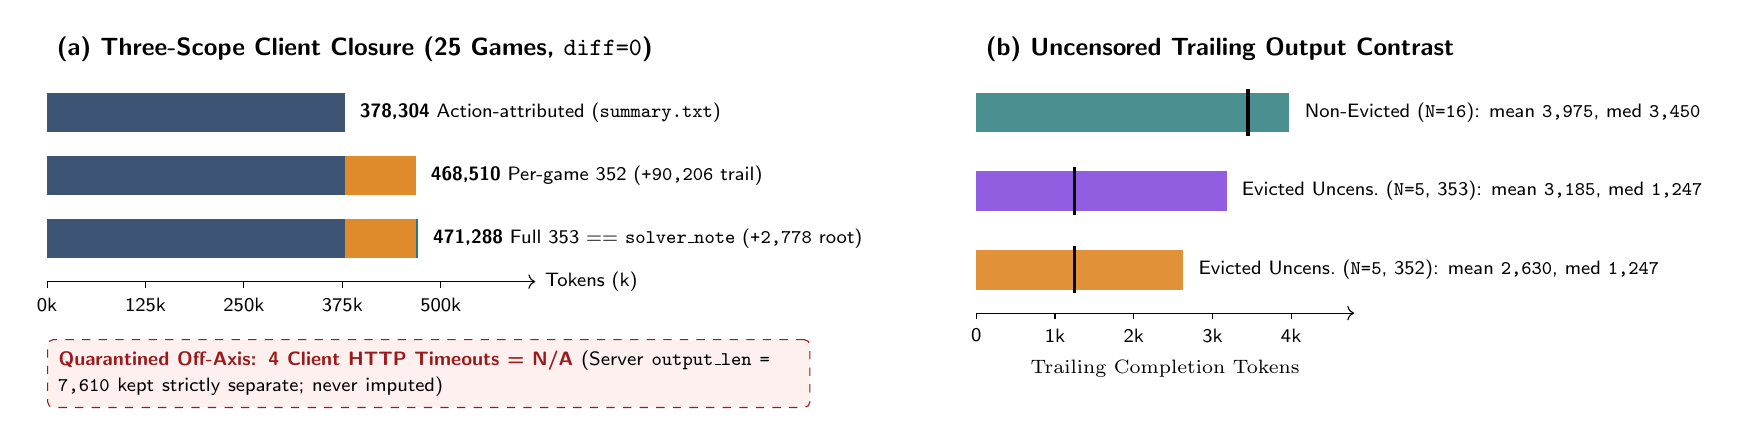
\begin{tikzpicture}[font=\sffamily\footnotesize]
\begin{scope}[xshift=0cm]
\node[anchor=west, font=\sffamily\small\bfseries] at (0,3.8) {(a) Three-Scope Client Closure (25 Games, \code{diff=0})};
\draw[->] (0,0.85) -- (6.2,0.85) node[right] {\scriptsize Tokens (k)};
\foreach \x/\lbl in {0/0, 1.25/125, 2.5/250, 3.75/375, 5.0/500} {
    \draw (\x,0.85) -- (\x,0.77) node[below] {\scriptsize \lbl k};
}
\fill[navy!85] (0,2.75) rectangle (3.783,3.25);
\node[anchor=west] at (3.85,3.0) {\scriptsize \textbf{378,304} Action-attributed (\code{summary.txt})};
\fill[navy!85] (0,1.95) rectangle (3.783,2.45);
\fill[accentorange!85] (3.783,1.95) rectangle (4.685,2.45);
\node[anchor=west] at (4.75,2.20) {\scriptsize \textbf{468,510} Per-game 352 (\code{+90,206} trail)};
\fill[navy!85] (0,1.15) rectangle (3.783,1.65);
\fill[accentorange!85] (3.783,1.15) rectangle (4.685,1.65);
\fill[tealdark!90] (4.685,1.15) rectangle (4.713,1.65);
\node[anchor=west] at (4.78,1.40) {\scriptsize \textbf{471,288} Full 353 == \code{solver\_note} (\code{+2,778} root)};
\node[draw=alertred, dashed, fill=red!6, rounded corners=2pt, anchor=north west, inner sep=4pt, align=left, text width=9.4cm] at (0,0.12) {\scriptsize \raggedright\textcolor{alertred}{\textbf{Quarantined Off-Axis: 4 Client HTTP Timeouts = \na{}}} (Server \code{output\_len = 7,610} kept strictly separate; never imputed)};
\end{scope}

\begin{scope}[xshift=11.8cm]
\node[anchor=west, font=\sffamily\small\bfseries] at (0,3.8) {(b) Uncensored Trailing Output Contrast};
\draw[->] (0,0.45) -- (4.8,0.45);
\foreach \x/\lbl in {0/0, 1.0/1k, 2.0/2k, 3.0/3k, 4.0/4k} {
    \draw (\x,0.45) -- (\x,0.37) node[below] {\scriptsize \lbl};
}
\node[anchor=north, font=\scriptsize] at (2.4,-0.02) {Trailing Completion Tokens};
\fill[tealdark!75] (0,2.75) rectangle (3.975,3.25);
\draw[very thick, black] (3.450,2.70) -- (3.450,3.30);
\node[anchor=west] at (4.05,3.00) {\scriptsize Non-Evicted (\code{N=16}): mean \code{3,975}, med \code{3,450}};

\fill[accentpurple!75] (0,1.75) rectangle (3.185,2.25);
\draw[very thick, black] (1.247,1.70) -- (1.247,2.30);
\node[anchor=west] at (3.25,2.00) {\scriptsize Evicted Uncens.\ (\code{N=5}, 353): mean \code{3,185}, med \code{1,247}};

\fill[accentorange!80] (0,0.75) rectangle (2.630,1.25);
\draw[very thick, black] (1.247,0.70) -- (1.247,1.30);
\node[anchor=west] at (2.70,1.00) {\scriptsize Evicted Uncens.\ (\code{N=5}, 352): mean \code{2,630}, med \code{1,247}};
\end{scope}
\end{tikzpicture}%
}
\caption{\textbf{Three-Scope Client Completion Accounting and Uncensored Trailing Gaps.} Panel~(a) closes \code{summary.txt}, per-game JSONLs, and \code{solver\_note} to exact zero discrepancy while moving censored \na{} timeouts cleanly off the token scale. Panel~(b) compares strictly uncensored episodes (\code{N=5} vs.\ \code{N=16}), displaying means (bars) and medians (vertical ticks).}
\label{fig:tokens}
\end{figure}

% ============================================================================
\section{Deterministic Context-Budget Eviction Replay and Prompt Mutation}
\label{sec:replay}

With client completion ledgers closed (\code{86.23\%} reasoning tokens), prompts grow rapidly toward \code{V10}'s context budget. Yet client event traces did not explicitly log when context pruning fired. Reconstructing exact eviction sites therefore requires opening the harness's online token estimator and prompt mutator.

\subsection{Why Character-Based Token Estimation and \code{[1.0, 3.3]} Clamping Exist}
Imagine packing a suitcase without a bathroom scale: you estimate bag weight from exterior volume, then recalibrate every time an airport check-in scale prints exact weight. Because the client harness sends raw strings/images to SGLang without running a full BPE tokenizer locally before every candidate truncation, \code{tool\_agent.py:3505--3509} allocates a target input token budget by subtracting the completion reserve and safety buffer from the configured \code{56K} window:
\begin{equation}
B_{\text{tok}} = \underbrace{57,344}_{56\text{K window}} - \underbrace{12,288}_{12\text{K reply}} - \underbrace{512}_{\text{margin}} = 44,544\text{ tok},\quad B_{\text{target}} = B_{\text{tok}} - \underbrace{16,384}_{\text{DRAIN}} = 28,160\text{ tok}.
\end{equation}
For text estimation, \code{\_calibrate\_from\_usage} (\code{tool\_agent.py:2903--2919, 5962--6008}) divides rendered payload character length by the latest observed server \code{prompt\_tokens} (after subtracting deterministic vision patch tokens) and clamps the resulting \code{chars/token} divisor $r_t$ to \code{[1.0, 3.3]}. As source comments note, \code{3.3} binds tightly on sparse game boards (\code{26/45} unique runtime emissions hit clamp limits) to err conservatively toward early trimming rather than server rejection. Forensic parsing across \code{77} files identifies \code{137} serialized occurrences corresponding to \textbf{\code{45} unique deduplicated emissions across \code{42} JSONL lines} (plus \code{2} \code{.log} emissions in \code{ft09} and \code{sk48}); deduplicating snapshot re-serializations is essential so \code{137} copies are never miscounted as \code{137} measurements.

\subsection{Two-Phase Prompt Mutation Mechanics (\code{Phase A} Image Scrub vs.\ \code{Phase B} FIFO Drop)}
When prompt estimates grow, Project HINAGI applies a deterministic \textbf{two-phase context cleaner} (Figure~\ref{fig:mutation} and Algorithm~2), analogous to cleaning an overflowing binder by first removing bulky photographs while keeping pages intact (\textbf{Phase~A}), and only tearing out the oldest chapters from the front if the binder still overflows (\textbf{Phase~B}):
\begin{itemize}[leftmargin=1.4em,itemsep=2pt]
\item \textbf{Phase A --- In-Place Image Scrubbing (\code{IMAGE\_KEEP=4}, \code{tool\_agent.py:6321}):} Once historical user messages hold more than 4 raster board images, \code{\_apply\_history\_image\_window} substitutes inline base64 payloads on older turns with short text placeholders. Message count stays unchanged, and \emph{only later prefix segments change} once scrubbing begins---a pattern occurring across \code{71} requests (\code{69} delivered) in \code{N=24/25} games (\code{bp35} excluded).
\item \textbf{Phase B --- FIFO Oldest-Turn Deletion (\code{L6323} \& \code{L6699}):} Whenever $\hat{T}_{\text{in}} > 44,544$, \code{\_trim\_\allowbreak messages\_\allowbreak for\_context} retains the system prompt (\code{$\sim$5,056} system+tool tokens) and drops the oldest \code{user}--\code{assistant}--\code{tool} groups until occupancy falls at or below $B_{\text{target}} = 28,160$ (\code{tool\_agent.py:6471}), cutting \code{ar25} from \code{44} messages down to \code{19}.
\end{itemize}

\begin{figure}[t]
\centering
\resizebox{0.96\textwidth}{!}{%
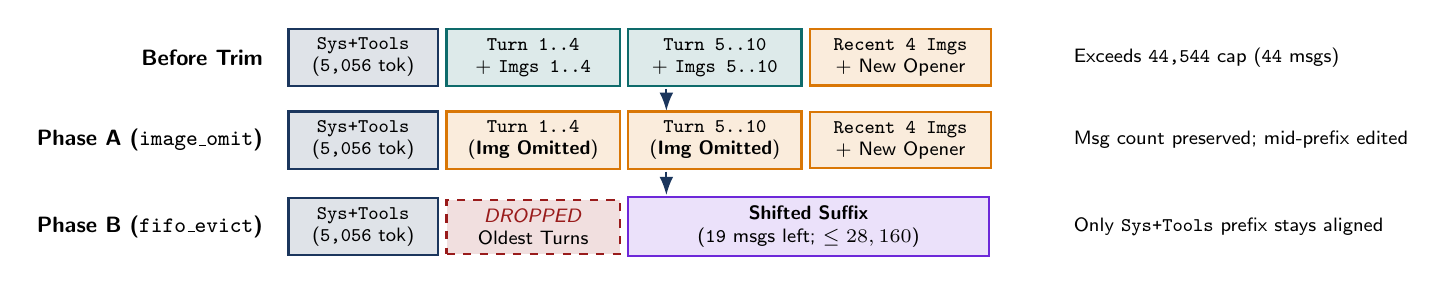
\begin{tikzpicture}[
    font=\sffamily\scriptsize,
    blk/.style={draw=#1, thick, minimum height=0.65cm, align=center, fill=#1!14},
    arr/.style={->, >=Latex, thick, draw=navy}
]
% Row 1: Pre-mutation
\node[anchor=east, font=\sffamily\footnotesize\bfseries] at (-0.2,2.2) {Before Trim};
\node[blk=navy, minimum width=1.9cm] (s0) at (0.95,2.2) {\code{Sys+Tools}\\(\code{5,056} tok)};
\node[blk=tealdark, minimum width=2.2cm, right=0.08cm of s0] (t1) {\code{Turn 1..4}\\+ \code{Imgs 1..4}};
\node[blk=tealdark, minimum width=2.2cm, right=0.08cm of t1] (t2) {\code{Turn 5..10}\\+ \code{Imgs 5..10}};
\node[blk=accentorange, minimum width=2.3cm, right=0.08cm of t2] (t3) {\code{Recent 4 Imgs}\\+ New Opener};
\node[anchor=west] at (9.85,2.2) {\scriptsize Exceeds \code{44,544} cap (\code{44} msgs)};

% Row 2: Phase A image_omit
\node[anchor=east, font=\sffamily\footnotesize\bfseries] at (-0.2,1.15) {Phase A (\code{image\_omit})};
\node[blk=navy, minimum width=1.9cm] (a0) at (0.95,1.15) {\code{Sys+Tools}\\(\code{5,056} tok)};
\node[blk=accentorange, minimum width=2.2cm, right=0.08cm of a0] (a1) {\code{Turn 1..4}\\(\textbf{Img Omitted})};
\node[blk=accentorange, minimum width=2.2cm, right=0.08cm of a1] (a2) {\code{Turn 5..10}\\(\textbf{Img Omitted})};
\node[blk=accentorange, minimum width=2.3cm, right=0.08cm of a2] (a3) {\code{Recent 4 Imgs}\\+ New Opener};
\node[anchor=west] at (9.85,1.15) {\scriptsize Msg count preserved; mid-prefix edited};

% Row 3: Phase B fifo_eviction
\node[anchor=east, font=\sffamily\footnotesize\bfseries] at (-0.2,0.05) {Phase B (\code{fifo\_evict})};
\node[blk=navy, minimum width=1.9cm] (b0) at (0.95,0.05) {\code{Sys+Tools}\\(\code{5,056} tok)};
\node[blk=alertred, dashed, minimum width=2.2cm, right=0.08cm of b0] (b1) {\textcolor{alertred}{\textit{DROPPED}}\\Oldest Turns};
\node[blk=accentpurple, minimum width=4.58cm, right=0.08cm of b1] (b2) {\textbf{Shifted Suffix}\\(\code{19} msgs left; $\le 28,160$)};
\node[anchor=west] at (9.85,0.05) {\scriptsize Only \code{Sys+Tools} prefix stays aligned};

\draw[arr] (4.8,1.80) -- (4.8,1.52);
\draw[arr] (4.8,0.75) -- (4.8,0.45);
\end{tikzpicture}%
}
\caption{\textbf{Two-Phase Context Trimming Mechanics (\code{Phase A} vs.\ \code{Phase B}).} Phase~A scrubs older inline raster frames (\code{IMAGE\_KEEP=4}) in place while preserving message count. Whenever estimates still cross \code{44,544} tokens, Phase~B deletes oldest conversational blocks from the head toward target \code{28,160}, leaving only the \code{5,056}-token system-and-tool header intact.}
\label{fig:mutation}
\end{figure}

\begin{conceptbox}{Algorithm 2: Deterministic Execution-Order Boundary Replay (\code{177/177} Parity)}
Replays \code{\_persistent\_history\_messages} (\code{L7184}) and \code{\_trim\_messages\_for\_context} chronologically per game:\\
1. At each request \code{c\_idx} opener (\code{tool\_agent.py:6699}), assemble \code{[sys] + history + opener}. If estimate exceeds \code{44,544}, mark \textbf{Next-Opener Trim (\code{L6699})} and pop oldest turn groups.\\
2. Update \code{chars/token} from delivered server \code{prompt\_tokens}, clamping to \code{[1.0, 3.3]}.\\
3. On turn exit (\code{L6321--6323}), prune resume messages, enforce \code{IMAGE\_KEEP=4} (\textbf{Phase~A}), and re-check \code{44,544}; if exceeded after image pruning, mark \textbf{End-of-Invocation Trim (\code{L6323})}.
\end{conceptbox}

\subsection{Why Turn-End Inspection Fails: \code{L6323} vs.\ \code{L6699} Replay \& Serialization Sensitivity}
Checking a checking account solely at midnight misses an overdraft triggered the next morning when rent debits arrive before a deposit. Similarly, auditing turn-end (EOS) snapshots alone misassigns \code{5} of the \code{9} evicted games:
\begin{itemize}[leftmargin=1.4em,itemsep=2pt]
\item \textbf{End-of-Invocation Trims (\code{tool\_agent.py:6323}, \code{4} games):} After applying the 4-image window at turn exit, estimates already exceeded \code{44,544} (\code{ar25} \code{44,748}, \code{ft09} \code{44,972}, \code{r11l} \code{52,276}, \code{sb26} \code{49,060}), shrinking history before the turn closed.
\item \textbf{Next-Opener Trims (\code{tool\_agent.py:6699}, \code{5} games):} At turn exit, estimates finished safely \emph{below} \code{44,544} (\code{bp35} \code{43,613}, \code{cd82} \code{43,223}, \code{cn04} \code{43,936}, \code{g50t} \code{42,523}, \code{vc33} \code{43,572} raw / \code{42,769} win-4 EOS), so nothing trimmed until appending the next step's \code{user} opener + image pushed the estimate over \code{44,544} (\code{44,645--45,993}). Near-miss game \code{tr87-cd924810} peaked at \code{44,318} open (\code{226} tokens under budget) and remained non-evicted.
\end{itemize}
Source-order execution of this dual-checkpoint state machine matches observed post-trim message counts across all \textbf{\code{177/177} post-initial steps} (Table~\ref{tab:eviction}). Because raw wire HTTP bytes were not logged, two auxiliary serialization scripts exhibit minor \code{19}--\code{400} token offsets (\code{44,645} vs.\ \code{45,045} on \code{g50t} depending on \code{tool\_choice} and image-window formatting). A sufficient invariance condition against an arbitrary serialization perturbation $\Delta_{\text{ser}} = 400$ tokens is $|\hat{T}_{\text{in}} - B_{\text{tok}}| > 400$. Auditing all \code{357} non-evicted/post-trim requests and all \code{9} pre-trim eviction triggers shows that \textbf{\code{174/177} (\code{98.31\%}) boundaries} lie strictly outside $B_{\text{tok}} \pm 400$: \code{7/9} evictions exceed \code{44,544} by \code{+428} (\code{ft09}) to \code{+7,732} (\code{r11l}) tokens, while among non-evicted requests only near-miss \code{tr87} (\code{44,318}, \code{-226}) falls inside the band (next closest: \code{43,389}, \code{-1,155}). Of the two evicted runs inside $\pm 400$, \code{g50t} Open (\code{44,645}, \code{+101} primary / \code{+501} secondary) and \code{ar25} EOS (\code{44,748}, \code{+204}) lie close to budget; however, \code{ar25} Open reaches \code{46,560} (\code{+2,016}), so even a \code{-400} shift only moves its trim site from \code{L6323} to \code{L6699} without changing eviction status, leaving \textbf{\code{175/177} (\code{98.87\%})} eviction classifications invariant.

\begin{table*}[t]
\centering
\caption{\textbf{Replayed Eviction Boundaries and Raw Provider \code{cached\_tokens} (\code{N=9} Evicted Games; \code{B\_tok = 44,544}).}}
\label{tab:eviction}
\resizebox{\textwidth}{!}{%
\setlength{\tabcolsep}{4pt}
\begin{tabular}{@{}l c l r r r r r l@{}}
\toprule
\textbf{Game ID} & \textbf{\code{c\_idx}} & \textbf{Trim Site} & \textbf{Msgs} & \textbf{Est.\ EOS} & \textbf{Est.\ Open} & \textbf{FIFO Prompt} & \textbf{Raw \code{cached\_tok}} & \textbf{Boundary Criterion \& Post-Trim Status} \\
\midrule
\code{ar25-0c556536} & 17 & \code{L6323} (End) & 44$\to$19 & \textbf{44,748} & 46,560 & 24,165 & 5,056 & $\text{EOS} > 44,544$; \code{11} post acts (\code{+1} level) \\
\code{ft09-0d8bbf25} & 13 & \code{L6323} (End) & 31$\to$17 & \textbf{44,972} & 46,814 & 27,056 & 5,056 & $\text{EOS} > 44,544$; \code{1} resp (\code{1,247} tok), \code{0} acts \\
\code{r11l-495a7899} & 12 & \code{L6323} (End) & 28$\to$14 & \textbf{52,276} & 53,944 & 27,403 & 5,056 & $\text{EOS} > 44,544$; \code{1} resp (\code{3,181} tok), \code{30.0s} TO \\
\code{sb26-7fbdac44} & 22 & \code{L6323} (End) & 55$\to$24 & \textbf{49,060} & 50,414 & 26,562 & 5,056 & $\text{EOS} > 44,544$; \code{1} post act, graceful exit \\
\midrule
\code{bp35-0a0ad940} & 14 & \code{L6699} (Open) & 32$\to$18 & 43,613 & \textbf{45,050} & 25,029 & 5,056 & $\text{EOS} \le 44,544 < \text{Open}$; \code{1} resp (\code{2,334} tok), \code{0} acts \\
\code{cd82-fb555c5d} & 14 & \code{L6699} (Open) & 36$\to$16 & 43,223 & \textbf{45,249} & \na{} (TO) & \na{} (TO) & $\text{EOS} \le 44,544 < \text{Open}$; \code{49.14s} TO (\code{srv\_out=1,928}) \\
\code{cn04-2fe56bfb} & 12 & \code{L6699} (Open) & 30$\to$17 & 43,936 & \textbf{45,993} & 26,297 & 0 & $\text{EOS} \le 44,544 < \text{Open}$; \code{3} acts, then \code{50.92s} TO \\
\code{g50t-5849a774} & 13 & \code{L6699} (Open) & 30$\to$7 & 42,523 & \textbf{44,645} & 12,650 & 5,056 & $\text{EOS} \le 44,544 < \text{Open}$; \code{1} act (\code{bF}), root \code{c\_idx=15} \\
\code{vc33-5430563c} & 18 & \code{L6699} (Open) & 44$\to$18 & 43,572$^*$ & \textbf{45,630} & 26,120 & 5,056 & $\text{EOS} \le 44,544 < \text{Open}$; \code{9} acts, then \code{30.0s} TO \\
\bottomrule
\end{tabular}%
}
\par\vspace{2pt}
\raggedright\scriptsize{$^*$\code{42,769} tokens after \code{win-4} image pruning at EOS (or \code{43,572} pre-window); near-miss \code{tr87} peaked at \code{44,318} open without triggering eviction.}
\end{table*}

% ============================================================================
\section{Prefix-Cache Stratification Under GPU LRU Unobservability}
\label{sec:cache}

\subsection{Why Host Mutations Trigger Prefix-Cache Cliffs (\code{RadixAttention} Mechanics)}
Consider printing a 100-page manual with reusable plates: appending Page~101 reuses Plates~1--100 cleanly, whereas deleting a figure on Page~15 or ripping out Chapters~1--5 shifts every downstream page alignment and forces fresh re-typesetting from that edit point onward. Because SGLang's \code{RadixAttention} \citep{zheng2024sglang} indexes GPU KV blocks by exact longest-common-prefix (LCP) token match starting from token index~0, we stratify all \code{357} client requests (\code{353} delivered full scope; \code{352} per-game scope) across four chronological transition states (Table~\ref{tab:prefix}, Figure~\ref{fig:prefix}):
\begin{itemize}[leftmargin=1.4em,itemsep=2pt]
\item \textbf{\code{pure\_append} (\code{251/252} delivered, \code{N=25} games, \code{0} zero hits):} Appending a new turn without editing prior history achieves \textbf{\code{88.52\%} pooled KV reuse} (\code{4,089,728 / 4,620,141}; \code{88.54\%} at \code{352} scope), with \code{87.74\%} game-pooled and \code{86.39\%} unweighted game means.
\item \textbf{\code{image\_omit\_mutation} (\code{69/71} delivered, \code{N=24} games excl.\ \code{bp35}, \code{16} zero hits):} Replacing older images alters mid-prompt tokens, co-occurring with a drop to \textbf{\code{15.53\%} pooled reuse} (\code{331,072 / 2,131,863}; \code{17.18\%} game-pooled / \code{17.03\%} game-unweighted).
\item \textbf{\code{fifo\_eviction} (\code{8/9} delivered + \code{cd82} timeout, \code{1} zero hit):} Deleting head turns breaks prefix matching immediately after the \code{5,056}-token shared system-and-tool header: \code{7} delivered runs reuse \textbf{exactly \code{5,056} tokens} (\code{ar25}, \code{bp35}, \code{ft09}, \code{g50t}, \code{r11l}, \code{sb26}, \code{vc33}), while \code{cn04} hits \textbf{\code{0}} (\code{35,392 / 195,282 = 18.12\%} pooled; \code{19.58\%} cluster mean).
\item \textbf{\code{initial} (\code{25} delivered, \code{N=25} games, \code{17} zero hits):} First requests average \textbf{\code{26.87\%} pooled reuse} (\code{40,576 / 151,030}: six \code{5,056}-token header hits, two \code{5,120}-token hits, and seventeen cold \code{0}s).
\end{itemize}
Combined, the \code{77} delivered \code{image\_omit\_mutation} and \code{fifo\_eviction} requests generate \code{1,960,681} uncached prefill tokens---\textbf{\code{75.37\%} of all uncached prefill computation} (\code{75.46\%} at \code{352} scope).

\begin{table*}[t]
\centering
\caption{\textbf{Clustered Prefix-Cache Stratification Across All \code{357} Requests (\code{353} / \code{352} Delivered Responses, with \code{10,000}-Iteration Game-Cluster Bootstrap 95\% CIs).}}
\label{tab:prefix}
\resizebox{0.99\textwidth}{!}{%
\setlength{\tabcolsep}{3.5pt}
\begin{tabular}{@{}l r r r r r r r c c@{\hspace{4pt}}}
\toprule
\textbf{Transition Class} & \textbf{Req} & \textbf{Deliv\,(353/352)} & \textbf{Games (\code{N})} & \textbf{Zeros} & \textbf{Prompt Tok} & \textbf{Cached Tok} & \textbf{Uncached} & \textbf{Pooled \% [95\% CI]} & \textbf{Game Mean (P/U) [95\% CI$_{\text{P}}$]} \\
\midrule
\code{pure\_append} & 252 & 251 / 250 & 25 & 0 & 4,620,141 & 4,089,728 & 530,413 & 88.52\% [87.38, 89.52] & 87.74\% / 86.39\% [86.48, 88.89] \\
\code{image\_omit\_mutation} & 71 & 69 / 69 & 24 & 16 & 2,131,863 & 331,072 & 1,800,791 & 15.53\% [12.65, 19.29] & 17.18\% / 17.03\% [14.04, 20.92] \\
\code{fifo\_eviction} & 9 & 8 / 8 & 8 (+1 TO) & 1 & 195,282 & 35,392 & 159,890 & 18.12\% [12.09, 23.88] & 19.58\% / 19.58\% [12.25, 27.11] \\
\code{initial} & 25 & 25 / 25 & 25 & 17 & 151,030 & 40,576 & 110,454 & 26.87\% [13.39, 43.62] & 26.87\% / 26.87\% [13.39, 43.63] \\
\midrule
\textbf{Host Mut.\ (\code{omit+fifo})} & \textbf{80} & \textbf{77 / 77} & \textbf{25} & \textbf{17} & \textbf{2,327,145} & \textbf{366,464} & \textbf{1,960,681} & \textbf{15.75\%} & \textbf{75.37\% uncached$^*$} \\
\textbf{Total (\code{353} Full)} & \textbf{357} & \textbf{353 / 352} & \textbf{25} & \textbf{34} & \textbf{7,098,316} & \textbf{4,496,768} & \textbf{2,601,548} & \textbf{63.35\%} & \textbf{\code{352}: 63.30\%} \\
\bottomrule
\end{tabular}%
}
\par\vspace{2pt}
\raggedright\scriptsize{$^*$Share of total uncached prefill tokens: \code{1,960,681 / 2,601,548 = 75.37\%} (\code{353} full) and \code{1,960,681 / 2,598,174 = 75.46\%} (\code{352} per-game). 95\% CIs resample whole game clusters ($N \in \{8,24,25\}$) with replacement ($B=10,000$, seed~42).}
\end{table*}

\begin{figure}[t]
\centering
\resizebox{0.96\textwidth}{!}{%
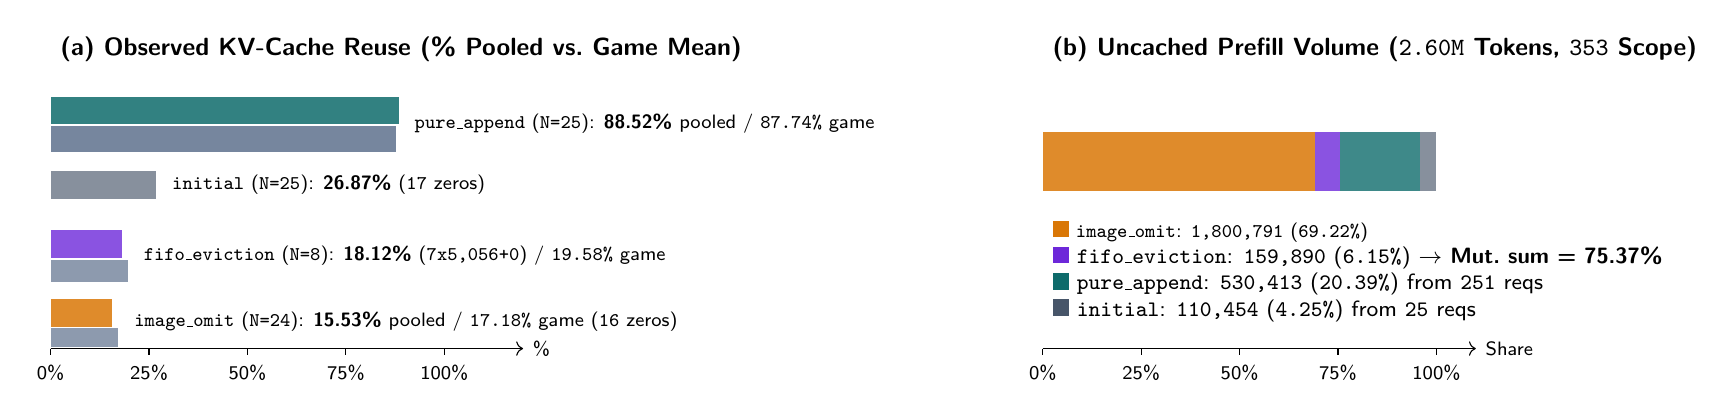
\begin{tikzpicture}[font=\sffamily\footnotesize]
\begin{scope}[xshift=0cm]
\node[anchor=west, font=\sffamily\small\bfseries] at (0,3.8) {(a) Observed KV-Cache Reuse (\% Pooled vs.\ Game Mean)};
\draw[->] (0,0) -- (6.0,0) node[right] {\scriptsize \%};
\foreach \x/\lbl in {0/0, 1.25/25, 2.5/50, 3.75/75, 5.0/100} {
    \draw (\x,0) -- (\x,-0.08) node[below] {\scriptsize \lbl\%};
}
\fill[tealdark!85] (0,2.85) rectangle (4.426,3.20);
\fill[navy!60] (0,2.50) rectangle (4.387,2.83);
\node[anchor=west] at (4.50,2.85) {\scriptsize \code{pure\_append} (\code{N=25}): \textbf{88.52\%} pooled / \code{87.74\%} game};
\fill[slate!65] (0,1.90) rectangle (1.344,2.25);
\node[anchor=west] at (1.42,2.08) {\scriptsize \code{initial} (\code{N=25}): \textbf{26.87\%} (\code{17} zeros)};
\fill[accentpurple!80] (0,1.15) rectangle (0.906,1.50);
\fill[navy!50] (0,0.85) rectangle (0.979,1.13);
\node[anchor=west] at (1.06,1.18) {\scriptsize \code{fifo\_eviction} (\code{N=8}): \textbf{18.12\%} (\code{7x5,056+0}) / \code{19.58\%} game};
\fill[accentorange!85] (0,0.28) rectangle (0.777,0.63);
\fill[navy!50] (0,0.02) rectangle (0.859,0.26);
\node[anchor=west] at (0.94,0.34) {\scriptsize \code{image\_omit} (\code{N=24}): \textbf{15.53\%} pooled / \code{17.18\%} game (\code{16} zeros)};
\end{scope}

\begin{scope}[xshift=12.6cm]
\node[anchor=west, font=\sffamily\small\bfseries] at (0,3.8) {(b) Uncached Prefill Volume (\code{2.60M} Tokens, \code{353} Scope)};
\draw[->] (0,0) -- (5.5,0) node[right] {\scriptsize Share};
\foreach \x/\lbl in {0/0\%, 1.25/25\%, 2.5/50\%, 3.75/75\%, 5.0/100\%} {
    \draw (\x,0) -- (\x,-0.08) node[below] {\scriptsize \lbl};
}
\fill[accentorange!85] (0,2.0) rectangle (3.461,2.75);
\fill[accentpurple!80] (3.461,2.0) rectangle (3.769,2.75);
\fill[tealdark!80] (3.769,2.0) rectangle (4.788,2.75);
\fill[slate!65] (4.788,2.0) rectangle (5.000,2.75);
\node[anchor=north west, align=left] at (0,1.75) {\scriptsize
    \textcolor{accentorange}{\rule{6pt}{6pt}} \code{image\_omit}: \code{1,800,791} (\code{69.22\%})\\
    \textcolor{accentpurple}{\rule{6pt}{6pt}} \code{fifo\_eviction}: \code{159,890} (\code{6.15\%}) \textbf{$\to$ Mut.\ sum = 75.37\%}\\
    \textcolor{tealdark}{\rule{6pt}{6pt}} \code{pure\_append}: \code{530,413} (\code{20.39\%}) from \code{251} reqs\\
    \textcolor{slate}{\rule{6pt}{6pt}} \code{initial}: \code{110,454} (\code{4.25\%}) from \code{25} reqs
};
\end{scope}
\end{tikzpicture}%
}
\caption{\textbf{Clustered Prefix-Cache Stratification Across Request Transitions.} Host mutations (\code{image\_omit} and \code{fifo\_eviction}) co-occur with sharp KV-cache drops and account for \code{75.37\%} of all uncached prefill tokens (\code{353} scope). Unlogged GPU RadixAttention LRU eviction events bar causal isolation.}
\label{fig:prefix}
\end{figure}

\subsection{Statistical Estimand Specification \& Cluster-Bootstrap Uncertainty}
Auditing the raw zeros reveals why we must exercise statistical restraint. Across \code{image\_omit\_mutation} (\code{16/69} zeros), \code{fifo\_eviction} (\code{1/8} zero on \code{cn04} despite an identical \code{5,056}-token header), and \code{initial} (\code{17/25} zeros), KV blocks vanish even at position~0 because concurrent 25-stream contention drives background GPU HBM LRU evictions that \code{serve.log} does not log. Furthermore, treating \code{n=69} or \code{n=251} intra-game requests as independent samples violates within-game serial dependence and makes request-level i.i.d.\ significance tests invalid. Using non-parametric game-cluster bootstrap resampling ($B=10,000$ iterations, fixed seed~42), \code{pure\_append} exceeds \code{image\_omit\_mutation} on paired game-pooled ratio means ($\Delta_P$, \code{N=24} games) by \code{70.48}\,pp (95\% CI \code{[66.08, 74.12]}\,pp; overall pooled contrast point estimate \code{72.99}\,pp [= \code{88.52\% - 15.53\%}], 95\% CI \code{[68.37, 76.18]}\,pp) and exceeds \code{fifo\_eviction} ($\Delta_P$, \code{N=8} games) by \code{68.79}\,pp (95\% CI \code{[61.21, 75.59]}\,pp; overall pooled contrast \code{70.40}\,pp [= \code{88.52\% - 18.12\%}]). Crucially, because \code{fifo\_eviction} spans only \code{N=8} delivered games forming a discrete step-function distribution (seven episodes pinned at exact \code{5,056}-token header hits and \code{cn04} at \code{0}), its bootstrap interval (\code{[12.09, 23.88]\%}) reflects non-asymptotic discrete resampling rather than a Gaussian approximation. Hierarchical request-level variance decomposition further shows that \code{90.9\%} of hit-ratio variance in \code{pure\_append} (\code{9.1\%} between-game) and \code{70.7\%} in \code{image\_omit\_mutation} (\code{29.3\%} between-game) occurs within episodes across turns, reinforcing why cluster-level inference is mandatory. Table~\ref{tab:estimands} codifies exact observation units (\code{N} games vs.\ \code{n} requests/actions), censoring rules, and cluster boundaries across every reported statistic.

\begin{table*}[t]
\centering
\caption{\textbf{Master Statistical Estimand, Observation Unit (\code{N} vs.\ \code{n}), Denominator, and Censoring Specification.}}
\label{tab:estimands}
\resizebox{\textwidth}{!}{%
\begin{tabular}{@{}l l l l l@{}}
\toprule
\textbf{Estimand} & \textbf{Unit} & \textbf{Numerator / Denominator} & \textbf{Censoring / Handling} & \textbf{Dependence \& Inference Bound} \\
\midrule
Client Token Closure (\code{S1/S2/S3}) & \code{N=25}, \code{n=353} & Sum of delivered \code{completion\_tokens} & 4 TO held \na{} (never pooled) & Exact deterministic sum (\code{diff=0}) \\
Uncensored Trailing Output & \code{N=5} vs.\ \code{N=16} & $\text{Comp}_{353} - \text{ActTok}$ & Excludes \code{4} timeout games & Descriptive contrast; endogenous length \\
Pooled Prefill KV Hit \% & Tokens (\code{n=353}) & $\sum \text{cached} / \sum \text{prompt}$ & Excludes \code{4} timeouts (\code{357$\to$353}) & Measures compute volume; not i.i.d.\ \code{n} \\
Cluster-Level Game KV Mean & Games (\code{N=24/25}) & Mean of per-game ratios (P / U) & \code{bp35} lacks \code{omit}; \code{cd82} TO & Primary unit (\code{N}); GPU LRU unlogged \\
Canonical V10 Public RHAE & \code{N=25} games & Weighted level RHAE (\code{Eq. 1}) & \code{0} missing; \code{16/25} zeros & 1-case distribution (\code{ft09=40.28\%}) \\
Unmatched Active Overlap & \code{N=10} V6-active & Sum/mean over \code{>0}-action overlap & Missing V6 JSONLs (\code{HOLD}) & Confounded \code{25} vs.\ \code{10} stream load \\
\bottomrule
\end{tabular}%
}
\end{table*}

% ============================================================================
\section{Qualitative Post-Eviction Failure Case Analysis (\code{N=9})}
\label{sec:recovery}

Having measured how FIFO deletion alters token budgets and prefix caching (Sections~\ref{sec:replay}--\ref{sec:cache}), we inspect where execution stalls or continues inside the \code{N=9} evicted \code{V10} cohort (\code{204} total physical actions: \code{179} Pre-Eviction actions, \code{16} Eviction-Step actions across \code{5/9} games, and \code{9} Strictly Later-Step actions concentrated in a single episode, \code{ar25}).

\subsection{Descriptive Case-Coding Checklist Across the \code{N=9} Cohort}
Because only \code{9} episodes crossed the Phase~B eviction boundary and only one episode (\code{ar25}, \code{1/9}) entered steps $t > t_{\text{ev}}$, these trajectories do not support a generalizable multi-stage law. Instead, we organize the observed failure and continuation points into a descriptive five-checkpoint case-coding checklist:
\begin{enumerate}[leftmargin=1.4em,itemsep=1pt]
\item \textbf{Check 1 --- Trim Boundary Entry:} Prompt crosses $44,544$ tokens and deletes head history (\code{PASS} for all \code{N=9} cases).
\item \textbf{Check 2 --- HTTP Response Delivery:} Trimmed and subsequent calls receive HTTP \code{200} usage rather than socket \code{ReadTimeout}.
\item \textbf{Check 3 --- Action Emission:} Model emits $\ge 1$ discrete physical environment action rather than terminating in prose.
\item \textbf{Check 4 --- Immediate Environment Progression (\code{EvStep}):} Actions within $t_{\text{ev}}$ yield valid board transitions (\code{bT}).
\item \textbf{Check 5 --- Cross-Step Continuity (\code{Later}):} Episode enters step $t > t_{\text{ev}}$ (\code{Later >= 1}), rebuilds persistent workspace state, and progresses cleanly (\code{0/9 bF} on \code{Later} steps).
\end{enumerate}

Table~\ref{tab:recovery} maps all \code{9} evicted games chronologically across these five descriptive checkpoints grounded in \code{events.jsonl} and \code{requests.jsonl}.

\begin{table*}[t]
\centering
\caption{\textbf{Descriptive Five-Checkpoint Case Coding of All \code{N=9} Post-Eviction Failure and Continuation Trajectories.}}
\label{tab:recovery}
\resizebox{\textwidth}{!}{%
\begin{tabular}{@{}l c c c c c c >{\raggedright\arraybackslash}p{4.8cm}@{}}
\toprule
\textbf{Game} & \textbf{Pre Acts} & \textbf{Check 2 (HTTP)} & \textbf{Check 3 (Emit)} & \textbf{Check 4 (\code{EvStep})} & \textbf{Check 5 (\code{Later})} & \textbf{WWM Post} & \textbf{Localized Failure / Continuation Profile} \\
\midrule
\code{cd82} & 10 & \textbf{FAIL} (\code{49.14s} TO) & FAIL (\code{0}) & \code{0} / \code{0 bF} & \code{0} / \code{0 bF} & 1 & Immediate Check~2 socket timeout on trimmed request \\
\code{bp35} & 8 & PASS (\code{1} resp) & \textbf{FAIL} (\code{0} acts) & \code{0} / \code{0 bF} & \code{0} / \code{0 bF} & 0 & Check~3 textual stall (\code{2,334} tok) before \code{stop} \\
\code{ft09} & 26 & PASS (\code{1} resp) & \textbf{FAIL} (\code{0} acts) & \code{0} / \code{0 bF} & \code{0} / \code{0 bF} & 0 & Check~3 textual stall (\code{1,247} tok) after 3 levels (\code{28.57}) \\
\code{r11l} & 10 & Partial (\code{30.00s} TO) & \textbf{FAIL} (\code{0} acts) & \code{0} / \code{0 bF} & \code{0} / \code{0 bF} & 3 & Check~3 non-action (\code{3,181} tok) then Check~2 timeout \\
\code{g50t} & 12 & PASS (\code{2+1} resps) & PASS (\code{1}) & \textbf{FAIL} (\code{1} / \code{1 bF}) & \code{0} / \code{0 bF} & 2 & Check~4 stagnant \code{DOWN} (\code{bF}) + root tail before \code{stop} \\
\code{sb26} & 33 & PASS (\code{2} resps) & PASS (\code{1}) & PASS (\code{1} / \code{0 bF}) & \textbf{FAIL} (\code{0}) & 0 & Executed 1 \code{MOUSE(22,22)} (\code{bT}) then terminated \\
\code{cn04} & 24 & Partial (\code{50.92s} TO) & PASS (\code{3}) & PASS (\code{3} / \code{0 bF}) & \textbf{FAIL} (\code{0}) & 2 & Executed 3 \code{RIGHT} (\code{bT}); aborted at Check~2 next step \\
\code{vc33} & 25 & Partial (\code{30.00s} TO) & PASS (\code{9}) & Partial (\code{9} / \code{1 bF}) & \textbf{FAIL} (\code{0}) & 2 & Retained Level-3 Phase-1 \code{9x MOUSE(56,46)} (9th \code{bF}); Step~10 TO \\
\midrule
\textbf{\code{ar25}} & 31 & \textbf{PASS} (\code{5} resps) & \textbf{PASS} (\code{11}) & Partial (\code{2} / \code{1 bF}) & \textbf{PASS (\code{9} / \code{0 bF})} & \textbf{4} & \textbf{Only Check~5 continuation (\code{1/9}):} rebuilt 4 world models, solved Level~2 \\
\bottomrule
\end{tabular}%
}
\end{table*}

\subsection{Side-by-Side Contrasting Cases: \code{ar25} Recovery vs.\ \code{vc33} Plan Exhaustion}
Comparing the two highest-action evicted trajectories clarifies what differentiates multi-step continuity from residual plan exhaustion:
\begin{itemize}[leftmargin=1.4em,itemsep=2pt]
\item \textbf{True Recovery (\code{ar25-0c556536}, \code{1/9}):} At Step~12 (\code{L6323}, \code{44 $\to$ 19} messages), \code{ar25} emits two \code{EvStep} moves (\code{RIGHT} \code{bT}, then \code{RIGHT} \code{bF}). Rather than halting, the agent reconstructs \code{4} working-world-model updates inside its persistent workspace across Steps~13--15 (\code{SPACE}/\code{LEFT} moves, then five \code{DOWN} actions with \textbf{\code{0/9} stagnant \code{bF} transitions} on \code{Later} steps), completing Level~2 (\code{score = 8.3333}) before graceful termination.
\item \textbf{Residual Plan Exhaustion (\code{vc33-5430563c}):} Having solved 2 levels (\code{9.4296}) and planned Level~3 Phase~1 prior to Step~9 (\code{L6699}, \code{44 $\to$ 18} messages), the surviving prompt suffix preserves the immediate Phase-1 coordinate recipe. The agent executes all \textbf{\code{9x MOUSE(56,46)}} actions in Step~9 (\code{8} \code{bT} followed by \code{1} stagnant \code{bF} at Action~34) before hitting a \code{30.00s} read timeout on Step~10 while trying to compute Phases~2--4.
\end{itemize}

% ============================================================================
\section{Bounded Quantitative Evaluation, Unmatched \code{Matched-10}, and Epistemic Quarantine}
\label{sec:eval}

\subsection{Local 25-Game V10 RHAE Distribution and Concentration}
Recomputing Eq.~\ref{eq:rhae} directly from action logs matches \code{benchmark.json} \code{final\_score} across all \code{50} local episodes (\code{V6} + \code{V10}) to machine precision (\code{max\_abs\_diff = 0.000000000000}). Canonical \code{V10} sums to \textbf{\code{70.937500}} (\code{mean = 2.837500}, sample \code{SD = 6.053709}, \code{median = 0.000000}, \code{IQR = 4.761905}), superseding earlier 2-decimal rounded summary totals (\code{70.93} / \code{2.8372}). Two structural properties constrain interpretation: (1) \textbf{\code{16/25 (64.0\%)} games score \code{0.0000}} with \code{0/25} full clears, and (2) single game \code{ft09-0d8bbf25} (\code{28.571429}) supplies \textbf{\code{40.28\%} (\code{40.2769\%})} of the entire 25-game sum (\code{remaining 24 mean = 1.7653}). Notice also that although the \code{Evicted} cohort averages higher (\code{6.5151} vs.\ \code{0.7688}), this reflects \textbf{endogenous length selection}: games that advance further survive more turns and therefore generate longer histories that reach the \code{44,544} trim limit.

\subsection{Resolving the \code{Matched-10} Concurrency Paradox Without Causal Claims}
Why does \code{V10} post a higher 25-game total (\code{70.94} vs.\ \code{49.84}) yet score lower (\code{-65.95\%}, \code{0W/6L/4T}) across the \textbf{\code{Matched-10} active overlap}---those 10 games where \code{V6} executed \code{>0} actions before its unreset boot clock expired? Imagine one water pump supplying 10 gardens (\code{V6}: 27 buckets each while 15 gardens sit dry) versus splitting the pump across all 25 gardens (\code{V10}: the first 10 drop to 13 buckets while 6 newly watered gardens sprout):
\begin{enumerate}[leftmargin=1.4em,itemsep=2pt]
\item \textbf{Stream Concurrency \& Action Volume Dilution:} In \code{V6} (\code{10} active streams, \code{TOOL\_STEPS=0}), GPU capacity concentrated on 10 games yielding \code{270} physical actions (\code{mean = 27.0}, \code{10} levels, \code{49.841270} RHAE). With \code{V10} activating all \code{25} streams (\code{TOOL\_STEPS=12}), action throughput across those same \code{10} games fell by \textbf{\code{-51.48\%} to \code{131} actions} (\code{mean = 13.1}, \code{16.969246} RHAE, \code{4} levels---e.g., \code{dc22} \code{35$\to$14}, \code{m0r0} \code{19$\to$7}, \code{tn36} \code{22$\to$6}, \code{wa30} \code{46$\to$16}, \code{lp85} \code{19$\to$11}, \code{vc33} \code{43$\to$34}), while allocating \code{255} actions (\code{53.9683} points) to the \code{15} previously starved games.
\item \textbf{Non-Evicted Loss Dominance:} Crucially, \textbf{\code{5 of 6} \code{V10} losses on \code{Matched-10} occurred in Non-Evicted games} (\code{dc22}, \code{lp85}, \code{m0r0}, \code{tn36}, \code{wa30}; only \code{vc33} experienced FIFO eviction). This pattern is observationally inconsistent with any hypothesis attributing the \code{Matched-10} score difference exclusively to FIFO eviction, while co-variation across \code{5/23} cells keeps the entire comparison strictly unmatched and non-causal (Table~\ref{tab:scores}, Figure~\ref{fig:matched}).
\end{enumerate}

\begin{table*}[t]
\centering
\caption{\textbf{Local Bounded Quantitative Evaluation (\code{V6} vs.\ \code{V10}, Unmatched \code{Matched-10}) and External \code{HOLD} / Offline Quarantine.}}
\label{tab:scores}
\resizebox{\textwidth}{!}{%
\setlength{\tabcolsep}{4pt}
\begin{tabular}{@{}l l r r r r r >{\raggedright\arraybackslash}p{5.0cm}@{}}
\toprule
\textbf{Run / Suite} & \textbf{Tier} & \textbf{\code{N}} & \textbf{Sum RHAE} & \textbf{Mean (SD)} & \textbf{Med (IQR)} & \textbf{Acts / Lv} & \textbf{Bounded Scope / Quarantine Note} \\
\midrule
\code{V6 Smoke} (all 25) & \code{E3-LOCAL-LOG} & 25 & 49.8413 & 1.9937 (4.63) & 0.00 (2.22) & 270 / 10 & \code{15/25} starved (\code{0} acts, \code{600.2--606.0s}); \code{0} wins \\
\code{V10 Local} (all 25) & \code{E3-LOCAL-LOG} & 25 & 70.9375 & 2.8375 (6.05) & 0.00 (4.76) & 386 / 13 & \code{16/25 (64\%)} zeros, \code{0/25} wins, \code{ft09=40.28\%} \\
\code{V10 Evicted Cohort} & \code{E3-LOCAL-LOG} & 9 & 58.6359 & 6.5151 (8.98) & 4.76 (8.33) & 204 / 10 & Endogenous length selection; \code{3} zeros \\
\code{V10 Non-Evicted} & \code{E3-LOCAL-LOG} & 16 & 12.3016 & 0.7688 (1.71) & 0.00 (0.00) & 182 / 3 & \code{13/16} zeros; \code{5/6 Matched-10} losses \\
\midrule
\textbf{\code{Matched-10}: \code{V6}} & \code{E3-LOCAL-LOG} & 10 & \textbf{49.8413} & 4.9841 (6.38) & 4.17 (4.21) & 270 / 10 & Unmatched active overlap (\code{10}-stream load, \code{TOOL=0}) \\
\textbf{\code{Matched-10}: \code{V10}} & \code{E3-LOCAL-LOG} & 10 & \textbf{16.9692} & 1.6969 (3.17) & 0.00 (2.08) & 131 / 4 & \textbf{Unmatched \code{0W/6L/4T} (\code{-65.95\%})}; \code{5/6} Non-Evicted \\
\midrule
Kaggle \code{57758308} (V6) & \textbf{\code{HOLD}} & --- & \holdbadge & \holdbadge & \holdbadge & --- & External payload absent from repo; zero citation \\
Kaggle \code{57827259} (V10) & \textbf{\code{HOLD}} & --- & \holdbadge & \holdbadge & \holdbadge & --- & \code{PENDING}/\code{null}; \code{TRUE\_SUBMISSION=True} disabled JSONLs \\
Kaggle \code{57912660} (V13) & \textbf{\code{HOLD}} & --- & \holdbadge & \holdbadge & \holdbadge & --- & Post-deadline external follow-up; zero citation \\
\code{Phase 6.0 / 6.4} & \code{E4-OFFLINE} & 25 & 260.3968 & 10.4159 (---) & --- & 0 LLM / 39 & Deterministic replay (\code{22/25} progressing, \code{1.425s}); non-LLM \\
\bottomrule
\end{tabular}%
}
\end{table*}

\begin{figure}[t]
\centering
\resizebox{0.96\textwidth}{!}{%
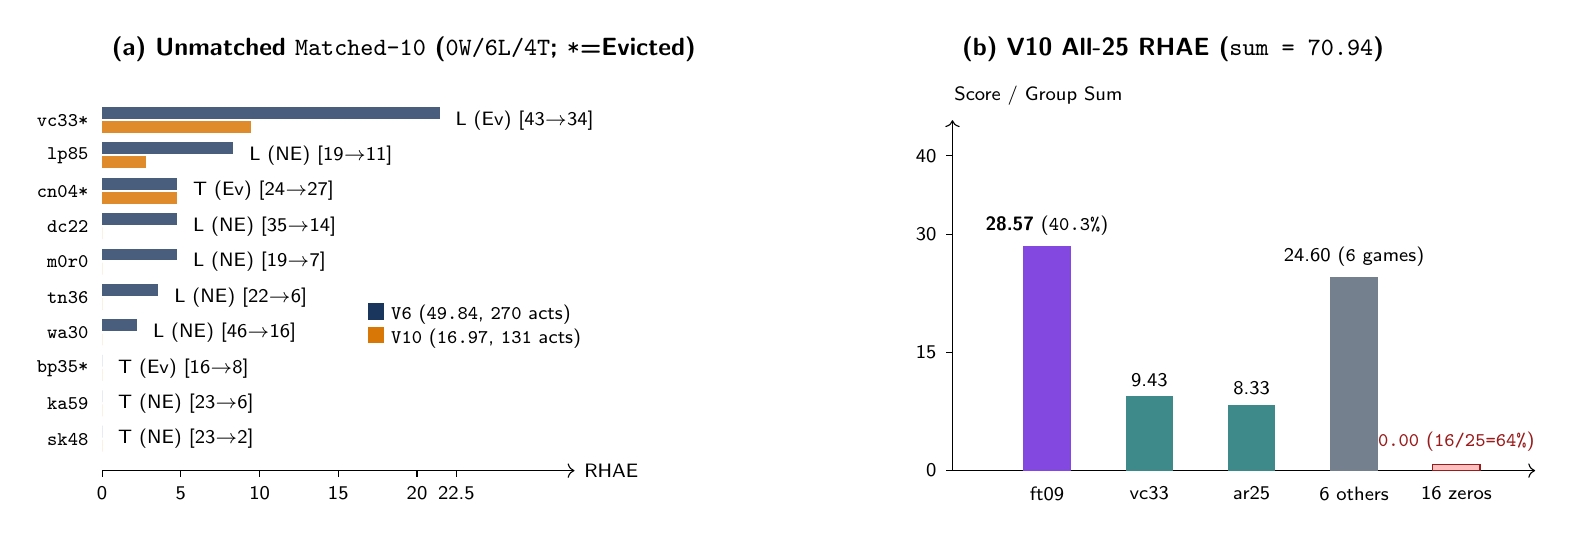
\begin{tikzpicture}[font=\sffamily\footnotesize]
% Left: Matched-10 Unmatched Active-Overlap Scores V6 vs V10 (Scale: 1cm = 5 RHAE)
\begin{scope}[xshift=0cm]
\node[anchor=west, font=\sffamily\small\bfseries] at (0,5.35) {(a) Unmatched \code{Matched-10} (\code{0W/6L/4T}; \code{*}=Evicted)};
\draw[->] (0,0) -- (6.0,0) node[right] {\scriptsize RHAE};
\foreach \x/\lbl in {0/0, 1/5, 2/10, 3/15, 4/20, 4.5/22.5} {
    \draw (\x,0) -- (\x,-0.08) node[below] {\scriptsize \lbl};
}
\foreach \idx/\g/\vvi/\vx/\reslbl in {
    1/vc33*/4.286/1.886/{L (Ev) [43$\to$34]},
    2/lp85/1.667/0.556/{L (NE) [19$\to$11]},
    3/cn04*/0.952/0.952/{T (Ev) [24$\to$27]},
    4/dc22/0.952/0.000/{L (NE) [35$\to$14]},
    5/m0r0/0.952/0.000/{L (NE) [19$\to$7]},
    6/tn36/0.714/0.000/{L (NE) [22$\to$6]},
    7/wa30/0.444/0.000/{L (NE) [46$\to$16]},
    8/bp35*/0.000/0.000/{T (Ev) [16$\to$8]},
    9/ka59/0.000/0.000/{T (NE) [23$\to$6]},
    10/sk48/0.000/0.000/{T (NE) [23$\to$2]}
} {
    \pgfmathsetmacro{\yy}{4.9 - 0.45*\idx}
    \pgfmathsetmacro{\barmax}{max(\vvi,\vx)+0.08}
    \node[anchor=east] at (-0.05,\yy) {\scriptsize \code{\g}};
    \fill[navy!80] (0,\yy+0.02) rectangle (\vvi,\yy+0.17);
    \fill[accentorange!85] (0,\yy-0.16) rectangle (\vx,\yy-0.01);
    \node[anchor=west] at (\barmax,\yy) {\scriptsize \reslbl};
}
\node[anchor=north west, align=left] at (3.25,2.25) {\scriptsize \textcolor{navy}{\rule{6pt}{6pt}} \code{V6} (\code{49.84}, \code{270} acts)\\[-1pt]\scriptsize \textcolor{accentorange}{\rule{6pt}{6pt}} \code{V10} (\code{16.97}, \code{131} acts)};
\end{scope}

% Right: V10 25-Game Score Concentration
\begin{scope}[xshift=10.8cm]
\node[anchor=west, font=\sffamily\small\bfseries] at (0,5.35) {(b) V10 All-25 RHAE (\code{sum = 70.94})};
\draw[->] (0,0) -- (7.4,0);
\foreach \x/\lbl in {1.2/ft09, 2.5/vc33, 3.8/ar25, 5.1/6 others, 6.4/16 zeros} {
    \node[below] at (\x,-0.08) {\scriptsize \lbl};
}
\draw[->] (0,0) -- (0,4.45) node[above=2pt, anchor=south west, xshift=-0.1cm] {\scriptsize Score / Group Sum};
\foreach \y/\lbl in {0/0, 1.5/15, 3.0/30, 4.0/40} {
    \draw (0,\y) -- (-0.08,\y) node[left] {\scriptsize \lbl};
}
\fill[accentpurple!85] (0.9,0) rectangle (1.5,2.857);
\node[above] at (1.2,2.86) {\scriptsize \textbf{28.57} (\code{40.3\%})};
\fill[tealdark!80] (2.2,0) rectangle (2.8,0.943);
\node[above] at (2.5,0.95) {\scriptsize 9.43};
\fill[tealdark!80] (3.5,0) rectangle (4.1,0.833);
\node[above] at (3.8,0.84) {\scriptsize 8.33};
\fill[slate!75] (4.8,0) rectangle (5.4,2.460);
\node[above] at (5.1,2.47) {\scriptsize 24.60 (\code{6} games)};
\fill[red!25, draw=alertred] (6.1,0) rectangle (6.7,0.08);
\node[above, text=alertred] at (6.4,0.12) {\scriptsize \code{0.00} (\code{16/25=64\%})};
\end{scope}
\end{tikzpicture}%
}
\caption{\textbf{Local Quantitative Evidence Boundaries and Concurrency Action Shifts.} Panel~(a) displays unmatched \code{Matched-10} active-overlap scores alongside \code{[V6 $\to$ V10 actions]}, showing \code{5/6} losses in Non-Evicted (\code{NE}) games under a \code{-51.48\%} action drop. Panel~(b) shows zero-inflated dispersion across all \code{25} \code{V10} games (\code{ft09} supplies \code{40.28\%}).}
\label{fig:matched}
\end{figure}

\subsection{External \code{HOLD} Quarantine \& Historical Lineage Errata Reconciliation}
Three hosted Kaggle submissions (\code{57758308} for V6, \code{57827259} for V10 with local status \code{PENDING} and \code{public\_\allowbreak score=null} under \code{TRUE\_\allowbreak SUBMISSION=True}, and post-deadline \code{57912660}) remain permanently quarantined in \code{HOLD} because raw API payloads do not exist on disk. Likewise, deterministic offline scripts (\code{run\_\allowbreak phase6\_\allowbreak 0\_\allowbreak vc33\_\allowbreak ablation.py} using hardcoded \code{ACTION6(46,56)} plus \code{StateConditioned\allowbreak Demonstration\allowbreak Memory}, and \code{run\_\allowbreak phase6\_\allowbreak 4\_\allowbreak matched\_\allowbreak evaluation.py} scoring \code{260.3968} over \code{25} games / \code{39} levels in \code{1.425s} with \code{0} LLM calls) are strictly isolated in \code{E4-OFFLINE}. Documenting two historical manuscript discrepancies reinforces this discipline: (1) two early \code{v6.4} repository PDFs carry divergent hashes and rank mentions (\code{194} in \code{branch\_a\_\allowbreak arcprize} vs.\ \code{189} in \code{submission/}) linked to \code{57758308}, both barred by \code{HOLD}; and (2) earlier \code{v6.4} prose mislabeled offline \code{Phase 6.0} replay as a ``controlled $2 \times 2$ ablation'', which R3.2 formally retracts and reclassifies as \code{E4-OFFLINE}.

% ============================================================================
\section{Systematic Related Work and Methodological Positioning}
\label{sec:related}

Re-opening systematic literature comparison across serving infrastructure, agent context engineering, evaluation methodology, and ARC agents allows humble calibration of our contribution (Table~\ref{tab:related}).

\paragraph{Prefix-Caching LLM Serving Systems.}
PagedAttention \citep{kwon2023pagedattention} (with vLLM's block-hashed Automatic Prefix Caching) and SGLang's RadixAttention \citep{zheng2024sglang} maximize multi-turn prefill efficiency by reusing KV blocks across identical leading token sequences under GPU LRU eviction. Both treat prefix preservation as a serving invariant; neither specifies a client-side execution-order boundary replay methodology to isolate client prompt edits (\code{image\_omit}, \code{fifo\_eviction}) when server logs omit internal GPU LRU eviction traces.

\paragraph{Agent Context Retention, Virtual Paging, \& Agent-Computer Interfaces.}
MemGPT \citep{packer2023memgpt} introduces OS-style hierarchical RAM/disk paging for unbounded conversations, SWE-agent \citep{yang2024sweagent} demonstrates how Agent-Computer Interfaces (ACIs) shape iterative error recovery, and \citet{lindenbauer2025complexity} reveal that simple sliding-window observation masking can match or beat LLM summarization on SWE-bench Verified without trajectory elongation. Our audit operates orthogonally one layer beneath high-level context policies: reconstructing calibrated client estimation clamping (\code{[1.0, 3.3]}), uncovering execution-order trim splits (\code{L6323} vs.\ \code{L6699}), and pairing context edits with KV-cache strata and qualitative post-eviction case profiles.

\paragraph{Agent Benchmark Rigor, Computational Reproducibility, \& ARC Agents.}
Kapoor et al.\ \citeyearpar{kapoor2025ai} expose cost neglect and reproducibility gaps in agent benchmarks, while CORE-Bench \citep{siegel2025corebench} directly evaluates scientific reproducibility agents. Our Evidence-Gated Auditing Protocol translates those normative standards into machine-verifiable runtime invariants (\code{diff=0} multi-scope closure, right-censored \na{} isolation, and \code{HOLD} quarantine).\footnote{We also examined an unindexed external technical manuscript on ARC-AGI-3 disk-backed workspace notes (\emph{ARC-Forge-2026}, Yi~Chia Chen and Simon Frieder, 2026) archived during internal design comparisons; because public web indexing and raw evaluation payloads are unavailable, it is omitted from quantitative bibliography comparisons and all internal judge/RL metrics remain excluded.}

\begin{table*}[t]
\centering
\caption{\textbf{Systematic Claim-by-Claim Literature Positioning Matrix Across Six Telemetry-Auditing Dimensions.}}
\label{tab:related}
\resizebox{\textwidth}{!}{%
\begin{tabular}{@{}l l c c c c c c@{}}
\toprule
\textbf{Work / System} & \textbf{Primary Domain} & \textbf{Multi-Scope Closure} & \textbf{Right-Censored TO (\na{})} & \textbf{Trim-Site Replay} & \textbf{Prefix vs.\ GPU Unobs.} & \textbf{Config Drift Quarantine} & \textbf{Post-Evict Rubric} \\
\midrule
PagedAttention / vLLM \citep{kwon2023pagedattention} & Serving KV Blocks & -- & -- & -- & Engine design & -- & -- \\
RadixAttention / SGLang \citep{zheng2024sglang} & Serving Prefix Tree & Partial & -- & -- & Engine LRU tree & -- & -- \\
MemGPT \citep{packer2023memgpt} & OS Context Paging & -- & -- & -- & -- & -- & Self-paging \\
SWE-agent \citep{yang2024sweagent} & Agent-Comp.\ Interface & Cost sum & -- & -- & -- & Controlled ACI & Error traces \\
Observation Masking \citep{lindenbauer2025complexity} & Context Compression & Turn tokens & -- & Policy level & -- & Controlled abl. & Trajectory len. \\
AI Agents That Matter \citep{kapoor2025ai} & Benchmark Validity & Normative & Calls for rigor & -- & -- & Critiques drift & Failure audit \\
CORE-Bench \citep{siegel2025corebench} & Reproducibility Eval & -- & -- & -- & -- & Artifact score & -- \\
\midrule
\textbf{This Work (V12 R3.2)} & \textbf{Telemetry Auditing} & \textbf{Yes (\code{diff=0})} & \textbf{Yes (Firewall)} & \textbf{Yes (\code{177/177})} & \textbf{Yes (Bounded)} & \textbf{Yes (\code{HOLD} / Diff)} & \textbf{Yes (Qual.)} \\
\bottomrule
\end{tabular}%
}
\end{table*}

% ============================================================================
\section{Limitations, Practitioner Guidelines, and Conclusion}
\label{sec:conclusion}

\subsection{Single-Case Scope, Threats to Validity, and Broader Impact}
\begin{itemize}[leftmargin=1.4em,itemsep=2pt]
\item \textbf{Internal Validity:} Five notebook cells (\code{Cells 0, 4, 6, 12, 16}) co-varied between \code{V6} and \code{V10}, \code{V6} lacks JSONL request traces, \code{serve.log} omits internal GPU RadixAttention LRU eviction events and per-step estimator state logs, and no \code{Guard-OFF} counterfactual exists. Accordingly, every cache contrast, config mechanism, and overlap regression remains strictly non-causal and observational.
\item \textbf{External \& Statistical Validity:} Empirical findings cover exclusively 1 harness, 1 quantized stack (\code{Qwen3.8-Flash-Next} W4A16 + SGLang), and 25 Public Split games (\code{64\%} zeros, \code{ft09=40.28\%}), and may not extrapolate to other models, benchmarks, or unseen competition splits (\code{HOLD}). Inference respects game clusters (\code{N=24/25}) via cluster bootstrap CIs rather than treating dependent intra-game requests (\code{n=69/353}) as i.i.d.\ draws.
\item \textbf{Methodological Implications:} Establishing transparent forensic telemetry auditing and right-censoring accounting reduces the risk of misattributing benchmark scores caused by silent infrastructure truncation, unlogged serving cache churn, or multi-variable launch drift. At the same time, deterministic audit compliance must never be misread as proof of general agent capability or causal hardware gains when serving LRU dynamics remain unlogged and sequestered competition splits remain quarantined in \code{HOLD}.
\end{itemize}

\subsection{Five Practitioner Design \& Telemetry Guidelines}
\begin{enumerate}[leftmargin=1.4em,itemsep=2pt]
\item \textbf{Prefer Prefix-Preserving Memory Policies Over Head FIFO Drops:} Head deletion forces recomputation past static headers (\code{7x5,056 + 1x0} pattern); isolate persistent workspace state outside conversational prefixes and trim strictly from appendable tails or summarized out-of-band buffers.
\item \textbf{Persist External Working World Models:} As illustrated by \code{ar25}'s post-eviction survival (\code{4} world-model rebuilds, \code{0/9 bF} later), storing compact structured state in a Python sandbox insulates agents when chat frames disappear.
\item \textbf{Emit Synchronized Dual-Plane Request IDs \& LRU Counters:} Always log exact request IDs alongside pre/post-trim message counts, online calibration divisors, and server-side GPU LRU eviction counters to close client--server observability gaps.
\item \textbf{Preserve Right-Censored Timeouts Explicitly:} Never replace client socket timeouts with zeros or mismatched server \code{output\_len} sums; report complete uncensored cohorts alongside censored rates (\code{N=5} vs.\ \code{4} timeouts).
\item \textbf{Enforce One-Factor Launch Controls:} Never co-vary server health-check timers, concurrency limits, tool depths, and pruning thresholds across experimental notebooks without single-factor ablations.
\end{enumerate}

\subsection{Conclusion and Future Work}
By re-engineering telemetry evaluation from scalar scoreboards into an \textbf{Evidence-Gated Auditing Pipeline}, we show how hidden prompt trims, client timeout censoring, prefix-cache collapses, and multi-cell launch drift explain apparent paradoxes in long-horizon visual tool agents without crossing causal or evidentiary boundaries. Future controlled hardware experiments (\code{Gate C}) should systematically cross budget size, media windowing, health-check isolation, and server LRU instrumentation under factorial randomization to isolate causal efficiency and reasoning trade-offs.

% ============================================================================
\appendix
\section{Code, Data, and Deterministic CPU Verification Availability}
\label{app:repro}

\paragraph{Public Release, Zenodo DOI, and Deterministic CPU Verification.}
All analysis code, unit tests, raw telemetry logs, and canonical verification ledgers are packaged in the public release \code{HINAGI\_R3\_2\_PUBLIC\_RELEASE} (distributed under the Apache License, Version~2.0 with \code{NOTICE}; historical \code{V12 R3.2-CP-3} and \code{Original Tier R1} baselines remain permanently preserved under the MIT License). Running \code{python3 verify\_tier\_r1.py} inside an isolated CPU clean room executes \code{141/141} manifest checks and all 7 deterministic replay stages in under 60\,s, confirming exact \code{diff=0} three-scope client token closure, \code{177/177} context-boundary replay, exact RHAE scoring parity, clustered prefix-cache aggregations across all 25 public games, and identical independent arithmetic JSON output (SHA-256 prefix \code{87fedfb1915f1bc6}). Upstream source traces in \code{reference/arc3\_franzen\_m2/} (\code{13/13} files) match \code{da-fr/arc-agi-3-solution} (commit \code{10882e33}, branched from \code{Tufalabs/duck-harness} commit \code{76528360}); the three Kaggle reference snapshot notebooks are preserved with co-retained Apache-2.0, MIT, and first-party notices. The public GitHub repository is hosted at \url{https://github.com/Heisnotanimposter/ARC-AGI-HIN} (release tag \code{v12-r3.2-public}, commit \code{d6079087c4b19dfd12f9db44f98e4709aff312ca}), and the permanent static archive is registered on Zenodo at \url{https://doi.org/10.5281/zenodo.24372990} (DOI \code{10.5281/zenodo.24372990}).

\paragraph{Historical Archive Lineage Errata.}
As summarized in Section~\ref{sec:eval}, two early unpublished \code{v6.4} manuscript variants in the development archive (\code{branch\_a\_arcprize} reporting Rank~194 vs.\ \code{submission/} reporting Rank~189) referenced external competition ID \code{57758308} and mislabeled deterministic offline \code{Phase~6.0} script replay as a ``controlled $2\times 2$ ablation.'' Both competition metrics remain quarantined under \code{HOLD} due to absent raw API logs, and \code{Phase~6.0}/\code{6.4} remain strictly isolated in \code{E4-OFFLINE} with zero live LLM claims. Furthermore, because server-side SGLang GPU RadixAttention LRU eviction traces were not emitted during the logged run, all prefix-cache contrasts remain strictly observational.

\section*{Acknowledgments and Funding Disclosure}
This research was conducted independently without external grant funding (self-funded). We acknowledge the authors of the upstream open-source inference harnesses audited and extended in this work: Jeroen Cottaar and Tufa Labs for \code{Tufalabs/duck-harness} (base commit \code{76528360}), and Daniel Franzen for \code{da-fr/arc-agi-3-solution} (commit \code{10882e33}, including the SGLang/harness patches), alongside J.~Pezzulli for \code{sglang-rtxpro6000}. AI coding and verification assistants (Antigravity and GPT) were used strictly as software engineering and audit-verification aids; the author bears full responsibility for all methodology, analysis, and conclusions.

\begin{thebibliography}{11}\small\setlength{\itemsep}{1pt}\setlength{\parskip}{1pt}

\bibitem[Chollet(2019)]{chollet2019measure}
F.~Chollet.
\newblock On the measure of intelligence.
\newblock \emph{arXiv preprint arXiv:1911.01547}, 2019.
\newblock \url{https://arxiv.org/abs/1911.01547}.

\bibitem[ARC Prize Foundation(2026)]{chollet2026arc3}
{ARC Prize Foundation}.
\newblock {ARC-AGI-3}: A new challenge for frontier agentic intelligence.
\newblock \emph{arXiv preprint arXiv:2603.24621}, March 2026.
\newblock \url{https://arxiv.org/abs/2603.24621}.

\bibitem[Kwon et~al.(2023)Kwon, Li, Zhuang, Sheng, Zheng, Yu, Gonzalez, Zhang, and Stoica]{kwon2023pagedattention}
W.~Kwon, Z.~Li, S.~Zhuang, Y.~Sheng, L.~Zheng, C.~H. Yu, J.~E. Gonzalez, H.~Zhang, and I.~Stoica.
\newblock Efficient memory management for large language model serving with {PagedAttention}.
\newblock In \emph{ACM Symposium on Operating Systems Principles (SOSP)}, 2023.
\newblock \url{https://arxiv.org/abs/2309.06180}.

\bibitem[Packer et~al.(2023)Packer, Wooders, Lin, Fang, Patil, Stoica, and Gonzalez]{packer2023memgpt}
C.~Packer, S.~Wooders, K.~Lin, V.~Fang, S.~G. Patil, I.~Stoica, and J.~E. Gonzalez.
\newblock {MemGPT}: Towards {LLM}s as operating systems.
\newblock \emph{arXiv preprint arXiv:2310.08560}, 2023.
\newblock \url{https://arxiv.org/abs/2310.08560}.

\bibitem[Zheng et~al.(2024)Zheng, Yin, Xie, Sun, Huang, Yu, Cao, Kozyrakis, Stoica, Gonzalez, Barrett, and Sheng]{zheng2024sglang}
L.~Zheng, L.~Yin, Z.~Xie, C.~Sun, J.~Huang, C.~H. Yu, S.~Cao, C.~Kozyrakis, I.~Stoica, J.~E. Gonzalez, C.~Barrett, and Y.~Sheng.
\newblock {SGLang}: Efficient execution of structured language model programs.
\newblock In \emph{Advances in Neural Information Processing Systems (NeurIPS)}, 2024.

\bibitem[Yang et~al.(2024)Yang, Jimenez, Wettig, Lieret, Yao, Narasimhan, and Press]{yang2024sweagent}
J.~Yang, C.~E. Jimenez, A.~Wettig, K.~Lieret, S.~Yao, K.~Narasimhan, and O.~Press.
\newblock {SWE-agent}: Agent-computer interfaces enable automated software engineering.
\newblock In \emph{Advances in Neural Information Processing Systems (NeurIPS)}, 2024.
\newblock \url{https://arxiv.org/abs/2405.15793}.

\bibitem[Kapoor et~al.(2025)Kapoor, Stroebl, Siegel, Nadgir, and Narayanan]{kapoor2025ai}
S.~Kapoor, B.~Stroebl, Z.~S. Siegel, N.~Nadgir, and A.~Narayanan.
\newblock {AI} agents that matter.
\newblock \emph{Transactions on Machine Learning Research (TMLR)}, June 2025.
\newblock \url{https://arxiv.org/abs/2407.01502}.

\bibitem[Siegel et~al.(2025)Siegel, Kapoor, Nadgir, Stroebl, and Narayanan]{siegel2025corebench}
Z.~S. Siegel, S.~Kapoor, N.~Nadgir, B.~Stroebl, and A.~Narayanan.
\newblock {CORE-Bench}: Fostering the credibility of published research through a computational reproducibility agent benchmark.
\newblock \emph{Transactions on Machine Learning Research (TMLR)}, 2025.
\newblock \url{https://arxiv.org/abs/2409.11363}.

\bibitem[Lindenbauer et~al.(2025)Lindenbauer, Slinko, Felder, Bogomolov, and Zharov]{lindenbauer2025complexity}
T.~Lindenbauer, I.~Slinko, L.~Felder, E.~Bogomolov, and Y.~Zharov.
\newblock The complexity trap: Simple observation masking is as efficient as {LLM} summarization for agent context management.
\newblock \emph{arXiv preprint arXiv:2508.21433}, 2025.
\newblock \url{https://arxiv.org/abs/2508.21433}.

\bibitem[Snell et~al.(2025)Snell, Lee, Xu, and Kumar]{snell2025scaling}
C.~Snell, J.~Lee, K.~Xu, and A.~Kumar.
\newblock Scaling {LLM} test-time compute optimally can be more effective than scaling model parameters.
\newblock In \emph{International Conference on Learning Representations (ICLR)}, 2025.
\newblock \url{https://arxiv.org/abs/2408.03314}.

\bibitem[Qiu et~al.(2026)Qiu, Wang, Li, Li, et~al.]{qiu2026qwen38}
Z.~Qiu, Z.~Wang, X.~Li, Y.~Li, et~al.
\newblock On the design of {Qwen3.8-Next} architecture: Evaluation, efficiency, and training stability.
\newblock \emph{arXiv preprint arXiv:2608.30320}, 2026.
\newblock \url{https://arxiv.org/abs/2608.30320}.

\bibitem[Pezzulli(2026)]{pezzulli2026pennyroyal}
J.~Pezzulli.
\newblock \code{sglang-rtxpro6000} (\code{pennyroyal-v253} serving stack).
\newblock GitHub repository \url{https://github.com/jpezzulli/sglang-rtxpro6000}, 2026.

\end{thebibliography}

\end{document}
